\documentclass[12pt]{report}
\usepackage{extsizes}
\usepackage[utf8]{inputenc}
\usepackage{graphicx}
\usepackage{lipsum}
\usepackage{listings}

\lstset{language=Python,
    % basicstyle=\scriptsize\ttfamily,
    % commentstyle=\ttfamily\itshape\color{gray},
    % stringstyle=\ttfamily,
    showstringspaces=false,
    breaklines=true,
    frameround=ffff,
    frame=single,
    % rulecolor=\color{black},
    xleftmargin=\dimexpr\fboxsep-\fboxrule,
    xrightmargin=\dimexpr\fboxsep-\fboxrule,
    gobble=8
}

\usepackage{verbatim}
\usepackage{float}
%Header and Footer Stuff
\usepackage{fancyhdr}
\usepackage{titlesec}
\assignpagestyle{\chapter}{fancy}
\pagestyle{fancy}
\fancyhead{}
\fancyfoot{}
\fancyfoot[R]{\thepage }
\renewcommand{\headrulewidth}{0pt}
\renewcommand{\footrulewidth}{0pt}
\usepackage[hidelinks]{hyperref}
\usepackage{graphicx}
\graphicspath{ {./images/} }
% \linespread{1.5}

\usepackage[lined,boxed,commentsnumbered]{algorithm2e}

% \usepackage{xr}
\usepackage{xr-hyper}
    \usepackage{hyperref}
    \externaldocument[chap01-]{sections/chapter01}
    \externaldocument[chap02-]{sections/chapter02}
    \externaldocument[chap03-]{sections/chapter03}
    \externaldocument[chap04-]{sections/chapter04}
    \externaldocument[chap05-]{sections/chapter05}
    


\title{Recommendation as a Balloon Debate}
\author{Harry Alexander Kelleher}
\date{April 2020}

\begin{document}

\pagenumbering{roman}

\begin{titlepage}
    \begin{center}
        
        \vspace*{1cm}
            
        \Huge
        \textbf{Recommendation as a Balloon Debate}
        
            
        \
        
            
        \vspace{2cm}
            
        \textbf{Harry Alexander Kelleher}
            
        \vfill
            
        Final Year Project\\
        BSc Computer Science\\
        Dr. Derek Bridge
            
        \vspace{0.8cm}
            
        
        \Large
        April 2020
    \end{center}
\end{titlepage}


\chapter*{Abstract}
    \addcontentsline{toc}{chapter}{Abstract}
    

    You are trying to decide which of the movies at your local cineplex to go and see. A recommender system can help you. In this project a Balloon debate recommender was created.  In a normal Balloon debate, a small number of speakers pretend to be famous people who are overloading the basket of a hot-air balloon. Someone must be thrown overboard. Each speaker gives reasons why they should be saved. An audience must decide who to sacrifice. 

    A set of movies compete against each other to see which one the cinema patron will pick. The movies can either be selected from current movies or movies the patron’s neighbours like. At the start of the debate, each movie explains why the movie should be kept. The patron then removes a movie based on the given explanations. In the next round, each movie gives a new explanation. This continues until a single movie is left standing. We have demonstrated refinement of choice using this methodology. 


\chapter*{Declaration of Originality}
        \addcontentsline{toc}{chapter}{Declaration of Originality}
        In signing this declaration, you are confirming, in writing, that the submitted work
        is entirely your own original work, except where clearly attributed otherwise, and
        that it has not been submitted partly or wholly for any other educational award. I
        hereby declare that:
        \begin{itemize}
            \item this is all my own work, unless clearly indicated otherwise, with full and proper accreditation;  
            \item with respect to my own work: none of it has been submitted at any educational institution contributing in any way to an educational award;
            \item with respect to another’s work: all text, diagrams, code, or ideas, whether verbatim, paraphrased or otherwise modified or adapted, 
            have been duly attributed to the source in a scholarly manner, whether from books, papers, lecture notes or any other student’s work, whether
            published or unpublished, electronically or in print.
        \end{itemize}
        \vspace{10mm}
        Signed: \dotfill Harry Alexander Kelleher \dotfill
        \\\\
        Date: \dotfill 17th April 2020 \dotfill


\chapter*{Acknowledgements}
    \addcontentsline{toc}{chapter}{Acknowledgements}
    I would like to thank Derek Bridge for all the help he has given during the project and giving me the chance to work on this project. He has been of tremendous help. I would like to thank my family for helping and providing support throughout this project. I would also like to thank all of the people who helped with beta testing the application and helped in user testing. 
   


\tableofcontents
    \thispagestyle{empty}
    

\listoffigures  
    \thispagestyle{empty}
    \addcontentsline{toc}{chapter}{List of Figures}

\lstlistoflistings
    \thispagestyle{empty}
    \addcontentsline{toc}{chapter}{List of Listings}



\chapter{Introduction}\label{sec:intro}
    \pagenumbering{arabic}
    

    \section{Recommender systems}
    
        Every year the amount of data created increases exponentially. Included in this increase is data such as movies and other online content. There is more and more media available to watch but the amount of time people have to spend watching this content is not increasing. Every year it becomes easier and easier for individuals to create their media content and share it on the internet. In 2001, 356 movies were released between the United States and Canada. The number of movies released each year has been increasing since then. The peak number was in 2018 when 878 movies were released. This is over a doubling since 2001. \cite{NumberOfMoviesReleased} This equates to two movies a day for an entire year. Most of these movies will not interest everyone, this problem can be mitigated by using movie recommenders. 


        The idea of movie recommenders is not new. Online streaming sites often include recommendation systems to help the user find the movies they want to quickly. Amazon and Netflix are the biggest movie streaming website and both have built-in recommendation engines that help users browse their websites. They do this because they have a huge backlog of content much of which will not be relevant to many people so as to not alienate customers they attempt to steer them in the right direction. When using these sites users get a curated selection of movies given to them. Sometimes these come with explanations as to why they should be chosen such as "We think you will like movie X as you have seen movie Y before. 
        They will also show you movie genres that are common between movies you have seen recently. The explanations for these movies recommendations rarely get more complex than if you like this movie you will like another. Although most streaming services contain a recommender I have not heard of a cinema that offers such services. In this project, we  plan to implement a recommender that will take movies from a local cinema and use them for recommendations. We will also explore creating a Netflix like recommender where we use more movies that just ones that are a local cinema.

    \section{Explanations}
        We want to solve the problem of a recommender not giving detailed enough explanations along with its recommendations. We want to explore creating a system that creates more explanations for a recommendation than, you might like X because you like Y. 
        It is assumed this is the case. We are going to use the assumption that if you like a movie and another user who like that movie might share other movies that you both might like. Therefore creating recommendations that we can show you. We can then use this movie and information about similar movies to create explanations tailored to you. We limited the project to recommendations based on movie ratings a user would provide the system. 


    \section{Balloon Debate}
        
        From our research, it appears seems that the concept of a recommender in the form of a debate has not been implemented. Where one speaker is removed per round. This gives the user some immediacy when playing the game as they feel they have to make a choice. This seems to be a novel approach that could give users an interesting experience while using a recommender. In our case the user  
        will have a selection of movies that are recommended to them. Each round they will be shown an explanation as to why they should keep that movie in the debate. After the user picks a movie to remove the next round begins and new explanations are shown. This continues until the user has only one movie remaining. There was an example of a recommender that took information created from a debate and used that to create recommendations for the user's friends \cite{10.1145/2792838.2799675}. This was similar to the planned project in  that it was a recommender that was more involved than picking a movie and explaining the reasons with other movies but ours will give recommendations in the game as apposed to using it to harvest data. Although what we are creating is a separate system that forms a game for a user to play. Pieces of the system could bae taken and implemented into a movie streaming site where movies are recommended and then explained using the above explanations. We  chose to structure the debate between six movies as that seemed like a good number where too few would not give enough rounds 


    \section{Project Overview}
        The aim was to accommodate a balloon debate between a set of movies where the user is the adjudicator. Movies currently being shown in the local cinema would compete against each other to be chosen by the user to see. Movies would give explanations as to why they should be picked and a user would be able to remove after each round of the debate. A system was created to do just this. The extent to which the movies can explain themselves was not decided in the outline but the system was extensible and more could be added. 
        
        In this chapter, we provided an introduction to the project and some background on why it is needed. In chapter 2 we will discuss some more background reading that is required for the project about recommender systems and about the work going into explaining the models created by artificial intelligence. We will also discuss the requirements for this project and what we hope to complete. In chapter 3 we are going to explore the creation of the recommender systems that were made in this project. In chapter 4 we are going to talk about the evaluation of the system where we created a user trial and invited people to test out the system and the results from the user testing. In the final chapter, we will talk about the conclusion of the project and some future work that could be undertaken. 
\chapter{Literature Review \& Goals} % 4 pages


    In this chapter, we are going to give an overview of the information that was acquired about recommender systems during the project and also include some explanations for things brought up in the design of the project. At the end of this chapter, we are going to explain the goals of the project before we describe the design for the recommender.

    \section{Information Filtering Systems}

        An information filtering system is a system that removes unwanted information. Nowadays there is so much media being created every day it can be very difficult to keep on top of everything coming out so it is very easy to miss movies you might be interested in. Recommender systems are a subset of Information Filtering systems.  A recommender system aims to predict the rating a user would give something based on some information it has. A recommender system aims to cut through all the extra data that exists now and bring you the most important information. Examples are the Netflix recommender that gives you an infinite list of movies you watch or Amazon's similar items recommender that gives you items other people like you, buy based on your purchase history. Major recommender systems can use either Collaborative filtering or Content-based filtering to create recommendations. 


    \section{Collaborative Filtering}
        Collaborative Filtering uses user behavior to link people together. This system does not use information or metadata about what you are recommending to make a recommendation. An example of this is the way \textit{Last.fm} recommends music to its users. It creates a station that plays music that people similar to you have played that you have not. They determine how similar you are to another user based on the common music tracks that you both listen to regularly. This has advantages that similar people are likely to listen to the same music so recommendations can be quite good. This type of recommender can be constrained by the cold start problem wherein the case of Last.fm the system needs to be seeded with a large amount of a users' music to be good at recommending. In this system, user taste can be acquired in different ways. It can be collected either implicitly or explicitly. You can collect data explicitly by asking users to rate pieces of data or using search results to form data points. You can also use information from other sources such as social media or their internet search results as implicitly collected data.


    \section{Content-Based Recommender}
        Another option for building a recommender system is to use content-based filtering. This is done using the information about what you are recommending instead of the users in the system. An example of this would be recommending music based on its metadata such as artist or the beats per minute of the song. If a user listens to songs that have a common bpm regularly it would make sense to recommend them more songs with that same bpm. This does not require as much seed data which means the cold start problem affects it less. The recommendations can be made more accurate the more information the system has. It can create more interesting connections between what a user has listened to and what they have not. 


    \section{Recommender System Problems}\label{sec:RecommenderSystemProblems}
        As we have mentioned above there are some problems that can be associated with certain types of recommenders. Collaborative filtering has problems such as the cold start problem and problems related to scalability and sparsity. Recommenders can have problems that are not created by the type of filtering they use.  

        \subsection{Cold Start Problem}
            When a new user signs up to a movie recommender that uses collaborative filtering it will be unable to create recommendations because it has no information about the user. As movies are added it will still be difficult to recommend anything until there is a significant amount of information that will allow the recommender to match you to other users that have similar viewing patterns. These types of recommenders need to be seeded with a set of ratings, to begin with in order to, recommend. This does not apply to recommenders that use Content-based matching as once you have one movie the system can start recommending based on that movie's metadata. This can be fixed by asking users to pull in information from other sources or by using a hybrid recommender that used multiple techniques. Movie lens \cite{10.1145/2827872} solves this problem by having users create a profile and then asking them to rate some movies as they create their profile so it is not empty.

        \subsection{Other problems}
            Scalability and Sparsity:
            As the size of a dataset increases the amount of computation necessary to calculate recommendations. Often recommending involves matrix calculations the size of the calculations increases the more examples and features involved. 
            If for example, the number of movies increases the matrices begin to get sparse meaning there will be lots of 0s in the dataset. This takes up space and does not help calculations. 


        \subsection{User Privacy}
            Recommenders are a fairly new invention. They were first mentioned in the year 1990 by Jussi Karlgren at Columbia University. He talked about them in relation to a "digital bookshelf". Nowadays most large websites that serve some form of content will have a recommender built-in. Google's search engine changes the results of the searches based on your history. YouTube will recommend videos based on a complex algorithm. Amazon has a recommender in the shopping website and integrated  into the streaming site Amazon prime video. Netflix and Spotify both have them. To create a recommender that can compete to today's standards involves collecting large amounts of data about all types of people to create good recommendations. Along with collecting large amounts of information comes the privacy concerns of what are these companies going to do with all this collected data. Some of these companies will go to great lengths to keep the algorithms as trade secrets. Once this data has been collected in can be used to create recommendations but also to swing elections. In the case of Cambridge Analytica who used data Facebook collected to target users with recommendations based on their data to swing their political views.
            
            As part of the growth of social media over the last 10 years, the recommendation of personalised content has grown with it. Part of the reason social media is so addictive is the endless scrolling through content that has been recommended to you. Websites like YouTube and Facebook keep you on their platform be trying their best to recommend a person content that will keep them there. In extreme cases, this can be detrimental to one's health as shown in \cite{SocialMediaAddiction}. As many recommender systems in these big websites are completely automated they often recommend any content that a user might like. This can lead to unsavory content being recommended to a user. Recommenders are supposed to just recommend the best content for a user so they are doing their jobs correctly. 
        
        

    \section{Correlation}\label{sec:pearsonCorrelation}
        As part of a collaborative-filtering recommender, correlation is often used to predict the relationship between users. Correlation is a statistical relationship between two variables. It can be used to predict relationships between data. It is a measure of the degree to which two variables are linearly related. For example, we can get the relationship between two people based on their movie ratings on a selected number of films. The most popular measure of the correlation between the two values is the Pearson Correlation Coefficient. It is defined as the quality of least-squares fitting to the original data, normalized to the square root of their variances. The Correlation Coefficient is just a measure of the correlation between the two values.  

        Correlations lie between -1 and 1. A value of -1 indicates that the two values are perfectly negatively linearly related. If the value is 0 this means there is no linear relation between the two variables although there might be a non-linear relation between the two values. There are examples of data and the produced Pearson Correlation shown in \ref{fig:PearsonCorrelationPic}

        \begin{figure}
            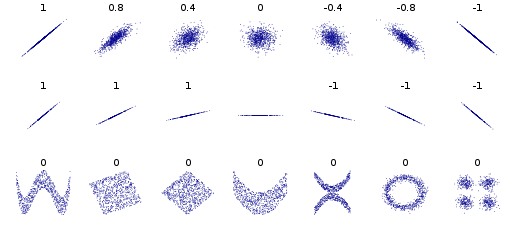
\includegraphics[width=125mm,scale=0.5]{PearsonCorrelation.png}
            \label{fig:PearsonCorrelationPic}
            \caption{Diagram showing various correlations Created by Denis Boigelot}
            \cite{PearsonCorrelationImage}
        \end{figure}

    

    \section{Explainable AI}
        In recent years there has been an effort to create explanations for recommendations that are created from artificial intelligence models. Explainable artificial intelligence is the section of AI that comes up with solutions to the problems relating to explaining the methods and techniques used in the application of AI technology. There are two types of models people use when creating artificial intelligence, white and black box models.  A model is a representation of a system that is created in order to understand the subject the model represents. In order to grow the trust that can be placed into models generated from artificial intelligence work has been done to increase their capacity to explain themselves. If they can explain themselves we are more likely to trust them. 

        \subsection{White Box Model}
            A white-box model is a model that is considered interpretable due to the simple structure. A small decision tree or sparse linear model are examples of this. Someone would be able to easily follow the selections down a small decision tree and it would be able to explain itself. A sparse linear model means many of the coefficients are 0. This leads to a model that is easy to understand as many of the features that are included in the prediction are not relevant. These often have a lower accuracy but have higher explainability. In figure \ref{fig:DecisionTreePic} we can see a decision tree. Starting at the top of the tree one can work their way down looking at the choice that was made at each stop helping to explain the decision. 


            \begin{figure}
                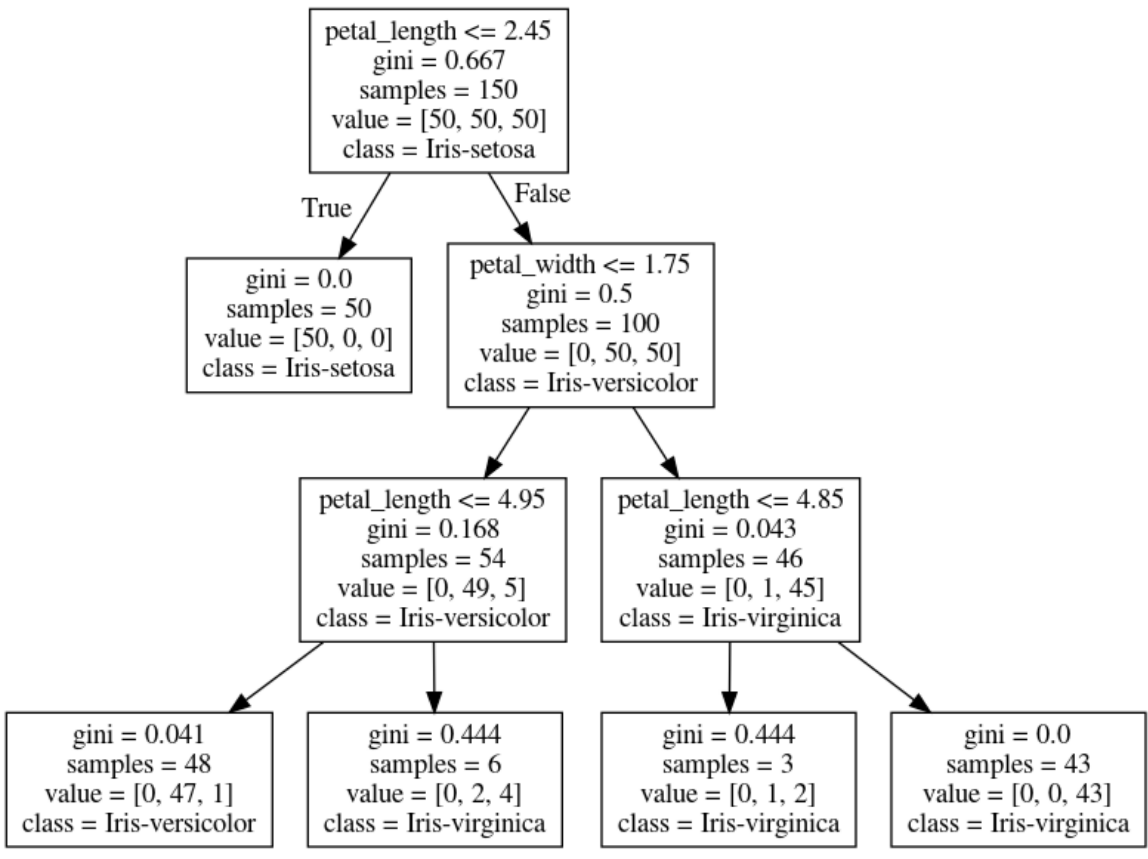
\includegraphics[width=125mm,scale=0.5]{DecisionTree.png}
                \label{fig:DecisionTreePic}
                \caption{Diagram showing a decision tree. Created by Derek Bridge  }
                \cite{DecisionTreeImage}
            \end{figure}


        \subsection{Black Box Model}
            A black box model on the other hand is a model where there is not an easy explanation that can be gathered. For example a neural network or ensembles such as Random Forests. A neural network is a system that is inspired by the neural networks in brains. These systems learn how to complete tasks based on examples given to them.
            Even big decision trees could be included in the black box model as it would be difficult for someone to discern an explanation from one as their size increases. Neural Nets are complicated enough that it would not be easy for a person to look through them and understand exactly how it came to its final decision using its weights. 


        \subsection{Explanation Methods}
            model-specific methods are methods of explanation that only work for a specific type of model. These can be made to work well for a single model but lack the ability to be general-purpose. Some methods only apply to decision trees for example LIME. LIME modifies the input data to a model and looks at the output in order to see what has changed. The output from LIME is a list of explanations that show the effect each feature of the input data had on the output. 

            Methods that work for any type of model are model agnostic. These are good because they are general purpose but often cannot  explain as well as model-specific methods as they have to work with more models.
            These have an advantage that they are much more flexible.
            There are many model-specific methods for explaining neural nets as they are popular and a type of black-box model.

        
    \section{Chain Based Recommenders}
        Another option for creating explanations for recommenders is the work done to create chain based recommendations \cite{Rana-Bridge-2017}. In this paper, they explored Recommendation by Explanation. In this system, they create a movie recommendation then get movies that are linked to that and create a chain. They then create explanations for the movies that are included in that chain. The Chain is created based on common keywords between the movies. This results in a high degree of serendipity, low population bias and high diversity. This is an interesting approach that seems to join a recommendation and an explanation. Conventionally these are considered separate tasks where recommendations are created and then explanations given.

    \section{Game-based Recommenders}
        \cite{10.1145/2792838.2799675}
        In this paper, they explore creating recommendations in a novel way. They have created a game with a purpose in order to solicit recommendations for movies.
        The game was hosted on Facebook so they could obtain information about the user likes their friends and what they like. This was then used to pick movies to include in the game. The player then has to pick the movies on the screen and assign them to a friend. This gets more difficult as the difficulty ramps up in the game. The answers from this could then be used to recommend a movie to a friend. They could then get the friends to rate the recommendations that were made satisfactory or not. Their results seemed to suggest this game was a better recommender than their collaborative filtering and content-based recommendation systems. 

    \section{Requirements}\label{sec:Requirements}
        in order to ensure the project matched what we planned we created a set of requirements both function and non functional that we could aim to complete.  
        \subsection{Functional Requirements:}
            \begin{itemize}

            \item The user must be able to search and rate movies to add to their profile.
            \item The user must be able to take part in user trials which accommodate a number of debates.
            \item The user should be able to view explanations for recommendations
            \item The user must be able to view the movies attached to their profile.
            \item The user must be able to view other users and the movies on their profile. 
            \end{itemize}
        \subsection{Non-Functional requirements}
            \begin{itemize}
                
            
            \item There must be a frontend for a user to interact with and there must be a single source where the data is stored. 
            \item The state of the user testing and the debates should be stored during operation.
            \item The user must be able to add their ratings to the system.
            \item The movies should create explanations for themselves. 
                \begin{itemize}
                    \item These may be scored relative to other explanations
                    \item Or they may be scored randomly for serendipity.
                \end{itemize}

            \item The system must be able to import information about new movies as they come out.
            \item The system should be able to compute the Pearson correlation between movies and users. 
            \end{itemize} 
\chapter{Design \& Implementation} % the next 4 chapters should be 40 ish pages

        
        

    \section{Introduction}
            The idea for this system was to create a website a user could interact with. To be able to make full use of the website the user should create a profile and rate a selection of movies. This will inform the recommender about their preferences. The user will participate in the debate and is shown a selection of movies from the local cinema. The recommender uses the information from the movies in the user's profile, as well as information about the recommended movies to create explanations that will be given during the course of the debate.

            Over the the project we created three systems. Each system was attempting to fulfil the same requirements although the first two were not successful, the third was. Each system was built on top of the previous using what was learned to create a better system. 

            Movies and their metadata are imported by the backend. Users sign up and create a profile this can then be filled with ratings. They can then start the debate. Movies are picked and their explanations created. The user can then participate in the debate by removing a movie after each round. Once this is completed they are left with one movie.


    \section{Schedule}
        At the start of the year, a set of goals for the project were laid out. The plan was to have the recommendation and explanations section of the project completed by the end of the first semester and to complete the debate and user interaction section in the second semester.\\


            \begin{tabular}{ |c|c| } 
                \hline
                September 27th      & Project started \\ 
                \hline
                October   10th      & Testing first system \\ 
                \hline
                November   20th     & Completed system to create explanations \\ 
                \hline
                November  30th      & Work slows in preparation for Christmas Exams \\ 
                \hline
                January 14th        & Start work on the debate and user interaction \\
                \hline
                March 1st           & Completed work on debate \\
                \hline
                March 10th          & Implement process for user trials\\
                \hline
                March 12th          & College Closed\\
                \hline
                March 26th          & Open Day (Cancelled)\\
                \hline
                April 1st           & User trials completed.\\
                \hline
                April 3rd           & Initial project end date (Postponed)\\
                \hline
                April 17th          & Project end as report due.\\
                \hline
            \end{tabular}
            
                    

    \section{First System}
        \subsection{Design}

            In this system, the user was presented with a command-line interface where the user would be asked which account to pick. These would be already existing accounts from the Movie Lens dataset. The system then picks 5 movies and gives back the average rating score for that movie. It would also search through the list of actors file and returns the actors that are linked to the movie. 
            It did give an explanation about a movie but was not based on a specific movie and was only one form of explanation and could not be easily extended. The interactions with the system from the user were limited to only supplying an already existing user id from the dataset. It was decided that actors was a good starting position for the movies and they are easily recognisable pieces of information about movies that people will cling to. For this project, we decided to use just user-supplied ratings from a dataset and the ratings users would provide during the use of the system. Other sources were considered, but implementing the collection of data from outside sources did not seem within the scope of the project, as the system only uses the fact the user has rated a movie, the ratings could be created from other data sources in an extended version of the project. 

        \subsection{Implementation}
            The first system was based of the Movie Lens and IMDB datasets. Movie Lens is a recommender website that suggests movies to users based on collaborative filtering of members' movie ratings. It was developed by GroupLens Research a research lab in the University of Minnesota. They offer a few different datasets. The first is a dataset designed for research that contains users with ratings on a scale of zero to five for a number of movies each. Each rating was a user id attached to a movie id and a rating. The dataset also contains a linking file between the movie ids that the Movie Lens dataset and the id system that the IMDB website uses. The movie ids from Movie Lens are not useful without the information to link them to the IMDB ids.
            
            The internet movie database referred to as IMDB \cite{IMDB} is the world's leading online repository for information about movies and other media. It launched in 1990 and is now owned by Amazon. It now contains over 6.5 million tiles made up of tv episodes, movies, video games and home media. It also contains over 10 million personalities. They supply subsets of their database online for people to use. We will be making use of the \textit{title.basic} and \textit{title.principals} datasets. These give information such as movie titles and their ids. It also gives actor information and links to the movies.

            This system would find some random movies from the dataset. Then for each movie it found it would get the average rating and also return the actors in it. For this we used the IMDB dataset. This contains a \textit{name.basics.tsv.gz} this contains 
            \begin{itemize}
                \item nconst (string alphanumeric unique identifier of the name/person) 
                \item primaryName (string name by which the person is most often credited)
                \item birthYear  (in YYYY format)
                \item deathYear (in YYYY format if applicable)
                \item primaryProfession (array of Strings)
                \item knownForTitles  movies the person is known for. 
            \end{itemize}
             A problem with this dataset is that it does not give all the movies the actor/actress was in only the ones they are known for, which reduces the usefulness of this. 

            \subsubsection{Development Tools}
                To start with the recommender only consisted of a command-line interface that was accessed by passing arguments to the Python scripts. This was sufficient for its purpose. Python was chosen for the project as we were familiar with it from previous assignments and a group project. It has many modules that can be imported to do anything that was going to be needed for this project. It is a general-purpose, high level interpreted language. The code produced is quite readable compared to other programming languages that we know. It is great for both small and large scale projects. It supports both functional programming and object-oriented programming, which we are going to use later in the project. It is dynamically typed and garbage collected. It also has a few other implementations that can be used for other advantages such as CPython which compiles Python code to bytecode for fast execution.
                
                We also started using Git which is a popular version control system developed by Linus Torvalds for use with managing the Linux Kernel. It designed for work in groups of people but is great for lone development as well. its goals are data integrity and speed and has support for distributed non-linear work. This is not a group project but I was working with multiple machines so having the git repo was very helpful. All code for the project was stored on Github which made working between machines possible. They provide hosting for software developers and were recently purchased by Microsoft. They also provide some code analysis which is useful for security vulnerabilities.
                
                Microsoft also makes VSCode which is a text editor come integrated development environment which has gained traction in the last few years. It was voted the most popular development environment in the Stack Overflow Development Survey where 50.7\% of respondents used the software \cite{StackOverflowDevSurvey}. It has built-in tools for git control and code completion. It also has a debugger that can be used with Python and Flask. 


            
        \subsection{Critique}
            This system was able to give explanations for the movies it was recommending to the user but the recommendations were not tailored and also not very relevant. The only information that the system would return is the average rating of the movie and the actors who appeared in it. This first system was a proof of concept and was used to learn about and get to know the two datasets. It was used to see what could be done with the datasets. This system did not meet most of the functional or non-functional requirements we had set out and so was used to form a new system that could be used to fulfil more requirements.
            This system was slow, had very limited user interaction as the user was just pretending to be an already existing user from the dataset and the presentation was lacking as it only have out information about actors.
                

        
    \section{Second System}
        \subsection{Design}
            After testing the usefulness of the data for explanations we decided we needed a way of creating them more easily. The initial idea for this system was to move to use a database to store all the information from the datasets this would speed up the access of the information in the system. The plan for the interactions was the same. The user would input a user id and would be given a set of actors based on information in their profile. A user would input a user id and the system would take this and compare this against ratings in the database. Taking all the movies from this user and then using the database to find all the actors for those movies. Ideally this would speed up the system and make it more useable. This system was going to be expanded to use all of the information that IMDB provide in their datasets; instead of just using actors to create explanations we were going to use more metadata about the movies. 

        \subsection{Implementation}
            Continuing on from the previous system, we wanted to implement something similar but with a database backend instead of searching the files. Keeping the same front end of inputting a user id and searching for some actors. Initially we started implementing SQLAlchemy models for each object in the system. The movies table was made up of 
            
            \begin{itemize}
                \item id       - INTEGER
                \item movie id - INTEGER
                \item name     - VARCHAR
                \item rating   - FLOAT
                \item IMDBid   - VARCHAR
            \end{itemize} 
            below you can see this translated into SQLAlchemy \ref{MovieClass}. This is a Movie class that can be instantiated in the code to create a new movie and then saved to the database as an item in the movies table. 
            

            \begin{lstlisting}[gobble=16, tabsize=4,caption=Representing the movie class,label=MovieClass]

                class Movie(Base):
                    __tablename__ = 'movies'
                    id = Column(Integer, primary_key=True)
                    movie_id = Column(Integer)
                    name = Column(String)
                    rating = Column(Float)
                    IMDBid = Column(String)

                    def __repr__(self):
                        return "movie_id='%i' name='%s'" % (
                            self.movie_id, self.name)
            \end{lstlisting}

            A similar thing was also implemented for some of the objects we were looking at putting in the system. An actor class was created with similar attributes swapping out IMDBid with the actor id and removing rating. This was then linked to the movie class using the class depicted in ~\ref{ActorToMovieClass}

            \begin{minipage}{\linewidth}
                \begin{lstlisting}[gobble=20, tabsize=4,caption=Representing the Actor to Movie class,label=ActorToMovieClass]

                    class Actor_to_Movie(Base):
                        __tablename__ = 'actor_to_movies'
                        id = Column(Integer, primary_key=True)
                        actor_id = Column(String,ForeignKey('actors.actor_id'))  # nconst 0
                        movie_id = Column(String, ForeignKey('movies.movie_id'))  # tconst 0

                        def __repr__(self):
                            return "<Movie_to_actor_paid(id='%i', actor_id='%s', movie_id='%s')>" % (
                                self.id, self.actor_id,self.movie_id)
                \end{lstlisting}
            \end{minipage}


            SQLAlchemy is an object-relational mapper which allows you to create an interface between items in a database and the objects in Python. Having developed with SQLAlchemy for our group project before it made sense to use it again for this project. This gives an interface in Python that can be used to create, edit, delete and search for items in the database using objects in Python. The problem with our use of this was that creating thousands of objects for inserting was going to take a long time. The plan was to take each piece of metadata and create a new Python object that would use SQLAlchemy to map to a table in the database. These classes have methods that can be used to add , update and remove each one. 
            


        \subsection{Critique}
            This system was not fully implemented as inserting the data from the datasets using SQLAlchemy was going to take a prohibitive amount of time. Instead, we moved onto system three which was also the final system. While using the IMDB dataset parsing all the files and linking the data became difficult so instead we moved to a different source of the information. 

        
    \section{Third System}
            \subsection{Design}

                The third system is made up of three parts. The first is obtaining movies and the data and importing it into the database. Next is taking that information and creating explanations with the movie and user information. In the third section, we will describe the user's interactions with the system and how it was presented to the user.


                \subsubsection{Collecting Movies}
                    In this system, we were continuing to use the user ratings from the movie lens dataset. These needed to be imported into our new database. We were unable to use the IMDB datasets as they do not contain all the information that we would like. Instead of using the IMDB datasets directly we are using the \textit{Open Movie Database}. This is an API created using some of the IMDB data as well as other sources. We were able to request data from this API to use. Combining the user ratings and the information from the API we were able to create a database of movies that we could create recommendations from. The application programming interface given by the Open Movie Database lets users specify the information required in the responses. 

                    The movies we are recommending in this system can come from two sources. Either they can come from the local cineplex or they are movies we are recommending to them based on their neighbour's ratings. Depending on the current debate we can either find the names of the movies from the local cinema by scraping the data or we can calculate which movies to recommend based on the user's Pearson coefficient between them and the other users in the system. As explained in \ref{sec:pearsonCorrelation} the Pearson correlation can be used to measure the similarity between two users. This is a form of collaborative filtering and can be used to get movie recommendations for users. We decided a choice many people have to make is what movie they want to see at their local cinema.The data that is collected from this section of the design can then be used to create explanations and debates.


                \subsubsection{Creating explanations}
                    After collecting movie information from the data sources and storing it. We need a system to create explanations. Based on the ratings that a user has we take every movie in their profile and collect all the common pieces of metadata between these movies and the movies that we are recommending. We gathered them we get the count of the number of times each piece of metadata appears in the user profile, this contributes to scoring the item. This creates a list of explanations we can give to the user. These are then scored and stored in the database. The scoring is done differently for each piece of metadata. 


                    Another form of explanation that the system uses is your neighbour's ratings. We calculate a user's top 50 neighbours based on the comparison between the user's ratings and the ratings of every other user in the system. Once a list of neighbours is created we can take the top 50 and show the ratings those users gave the movie we are recommending. Depending on the piece of metadata the scoring is done by comparing how often an item appears in the database of movies in the system versus how many times it appears in the user's profile. The higher the better as we are assuming for example that if a user has seen an actor in many films they might be likely to want to see them again. 


                    \subsubsection{User interaction}\label{sec:3UserInteractionDesign}
                    To interact with the system the user will go to one of a few pages after they have created an account and logged in. There is a page where a user can import a new movie by supplying its name or IMDB id and give it a rating on that page. This will use the importer to import the movie and add the rating to the user's profile. There is also a page to rate any existing movie in the system. The user is presented with a selection box of all the movies in the system and another to select a rating between zero and five. If the user has already rated the movie we update their rating. On this page are the controls for the user trials and the debates. The user can start the user trials. This has six rounds, each has different settings for creating recommendations and explanations. The user is able to start the trials and advance them from this page. There is also the showings page which was used for testing. This page lets the user see all the current movies and all their explanations attached without needing to go to the debate.

                    Initially, the user trials were going to be done in person, where we could change the settings as the user completed debates. As the College was closed due to the COVID-19 pandemic, a new system had to be created. The user trials are explained in chapter \ref{sec:userTrials} The final page the user can visit is the debate page. On this page the user sees the six movies that are being recommended to them along with the explanations underneath. The movies are represented by their title and a poster.  There is a movie selection box at the bottom of the page that lets users remove a movie each round. The system will also need to be hosted so that users will be able to access it. The plan is to host the system publicly from home as this is the cheapest and easiest method. 

        
                    \begin{figure}
                        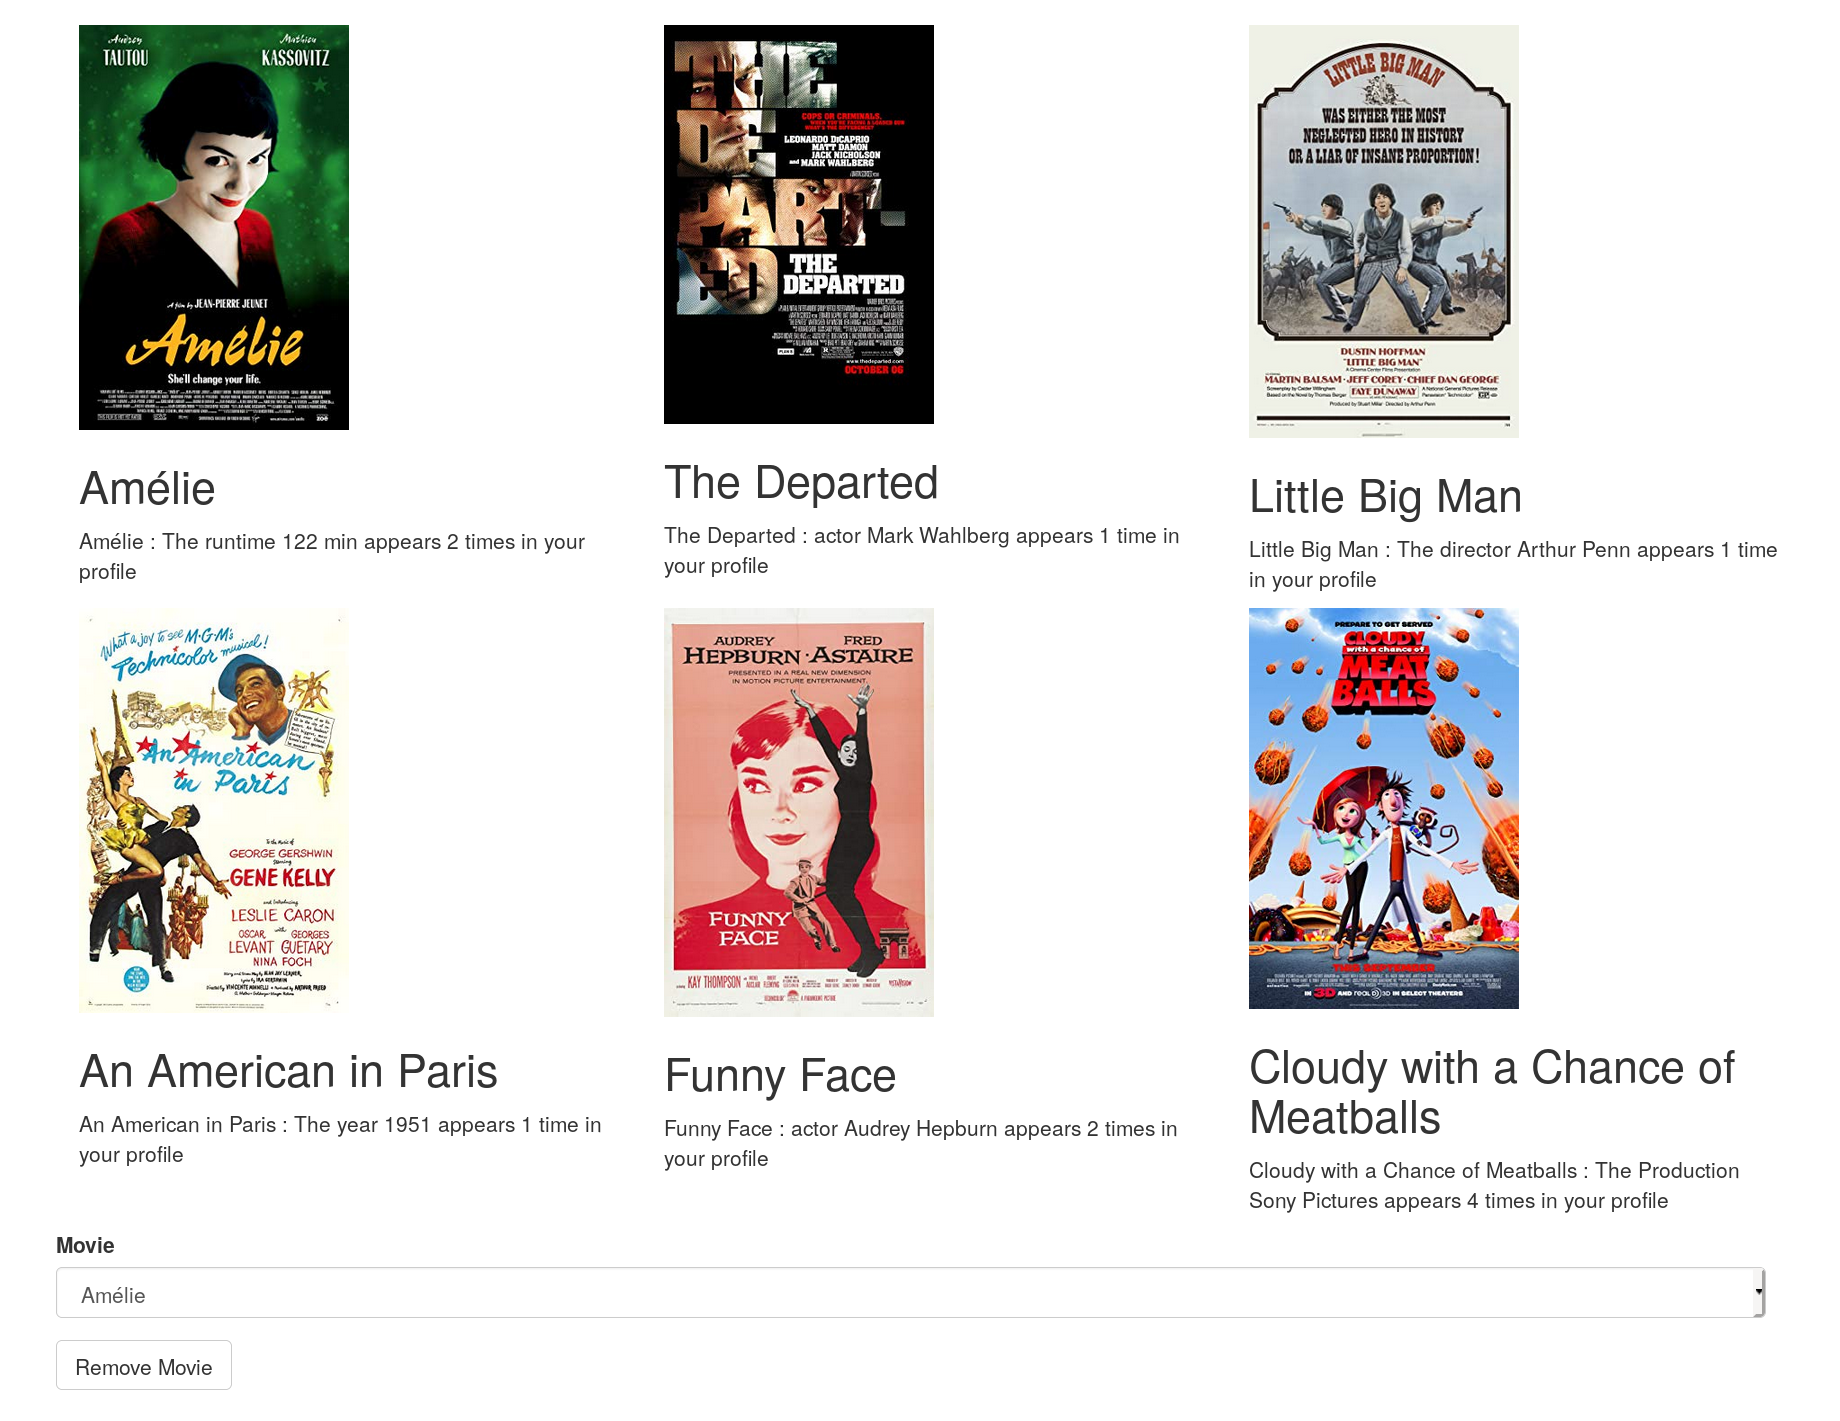
\includegraphics[width=125mm,scale=0.5]{system1.png}
                        \caption{The debate screen of the application}
                    \end{figure}

        
                    \subsubsection{Critique}
                        Ideally the system would not use just a user's movie ratings. It would use some less specific ratings of a system. \cite{10.1145/1555400.1555432}. In this paper, it is seen that users are likely to not want to rate movies explicitly. If the system was used inside another system, the user preferences could be calculated based on things other than ratings. Such as the watch list of a user or the movies they have looked at on an interface but not watched. We could also deem a negative rating of a movie a user started to watch but stopped and never came back. To create explanations we just looked at all of the movies a user had rated and took objects they had seen frequently and explained the recommendation using these. The scoring of these explanations did not take into account if the object was taken from a movie the user disliked. The scoring for explanations could have been made better if it took into account the actor they that was being used as an explanation was from a movie the user did not like.

            \subsection{Implementation}
                \subsubsection{Collecting Movies}\label{sec:CollectingMovies}
                    To be able to create recommendations and explanations we were going to need a database of movie information. Instead of using the IMDB datasets which do not give the information we want. The information we would like would have to be created by a system we create.  We started using the Open Movie Database API. 

                    "The OMDb API is a RESTful web service to obtain movie information, all content and images on the site are contributed and maintained by our users."\cite{OpenMovieDatabase} This can be accessed online or through one of a few different Python wrappers. You can supply an IMDB id or a title and it will give you back structured data about the movie similar to what the IMDB datasets can provide but easier to parse. This gives more information than IMDB provide in their datasets and also gives posters. The user can then specify what type of content they want from the API with different parameters when they make the request. There is a module that has been created called OMDb \cite{pythonOmdbApi}

                    As part of wanting to create the database for user and movie information we needed to decide on which database to use. There are many options for this. We decided on using SQLite. It is a relational database management system that instead of using the standard client-server model, it instead uses a function library that can be called from the application. SQLite is file-based. SQLite is considered simpler than MySQL which is a standard client-server DBMS. Using MySQL would have increased the complexity of the project. It would have involved running a MySQL server alongside the application. MySQL can be much faster in some cases but through the use of SQLite transactions we can reduce the difference and make SQLite faster. Another popular option is PostgreSQL which is open source and has some advantages like the ability to deal with a great number of concurrent clients. 

                    In order to collect movies, we can take a movie id from the movie lens user ratings and query the api and it will give us back JSON that can be split up and inserted into the database. Each object has its own table, for example actors and directors. These are all represented as an object id and a string. There is a table that shows, for each movie, all of the objects attached to that movie. The code in figure \ref{lst:InsertingMovies} shows how we take the information that the OMDb Python library returns and use it to create new objects. 

                        \begin{minipage}{\linewidth}
                            \begin{lstlisting}[gobble=32,tabsize=4,caption={Importing movies into the database},label={lst:InsertingMovies},language=Python]
                            
                                def import_movie(IMDB_id):
                                    json_for_movie = omdb.IMDBid(IMDB_id)
                                    response = literal_eval(json_for_movie)
                                    movie = response["IMDB_id"]
                                    for object in response:
                                        if check_exists(object):
                                            pass 
                                        else:
                                            create_object_and_insert(object)
                                            create_movie_object_link(object,movie)
                            \end{lstlisting}
                        \end{minipage}
                      

                    The names of movies that are going to be recommended can come from two sources. The first is movies that are being shown at the local cinema and the other is movies the user's neighbours have rated highly. 

                    In order to get a list of movies from the local cinema we create a function \textit{get\_omniplex\_movies()} . This would make requests to the website and retrieve a list of movies formatted in such as way that would be usable to us. We used the Python requests module to make requests to the website. The website would not return a list of movies unless we used a valid request with the correct headers. We included the standard headers that would be given if you were using a web browser to access the page and retrieved the list of titles that were needed. This cinema has showings for more than just movies so these needed to be filtered out manually as there was no way to request just a list of movies that would work with the system. This was done mainly as the API we were using for movie metadata would not contain these other showings. We would therefore not be able to make explanations for them so they were excluded. \textit{Beautiful Soup 4} was used to parse the returned HTML. This is a Python library for pulling data out of HTML and XML files. It provides an easy way to parse the HTML. 

                    
                    To calculate a users neighbours we used the Pearson correlation coefficient. Using this we can get a measure of the similarity between two user's ratings. Initially, we were going to create neighbours based on the threshold of the relationship between them but a better practice is to use a limit on the number of neighbours and for example take the top 30 nearest neighbours. \label{sec:CreateNeighbours}

                    \subsubsection{Calculate Pearson Coefficient}
                
                        To calculate the Pearson coefficient for our users we used the Scipy stats module. This provides a function \textit{pearsonr(a,b)} which takes in two lists and returns the coefficient and the p-value. If either of the lists is a list composed of all the same values the function will return nan. This is because you cannot calculate variance in a list of the same numbers as they do not vary which would lead to trying to divide by zero in the formula. In our implementation, we assumed the coefficient was zero between two lists if one of the lists was composed of only one value repeated.
                        
                        First the function in \ref{fig:FindingNeighboursPearsonMethod} finds all of the possible neighbours. This is anyone who has rated at least one movie that the user has also rated. Then we find every movie a possible neighbour and the user share. When run, the SQL shown in \ref{fig:FindingNeighboursPearsonMethodSQL} returns a list of pairs of ratings. Each pair is the rating for a movie that is shared between two users. The pearson correlation is calculated between the two lists. This is done for each neighbour and the results are sorted and ranked. The fifty neighbours with the highest correlation with the user are used as the neighbours.

                        Assuming $\bar{x}$ is the mean of list x , $\bar{y}$ is the mean of the list y and that $s_x$ and $s_y$ are the std deviation of list x and list y you can use these to calculate the coefficient. For each value in each list, you need to calculate a standardised value using $(z_x)_i$ and $(z_y)_i$ for lists x and y respectively. For  each of the standardised values you can multiply them together then add them together and divide by n-1 where n is the length of the lists. This results in the Pearson coefficient between lists x and y.

                        \begin{minipage}{\linewidth}
                            \begin{lstlisting}[gobble=30, tabsize=4, caption=SQL used to find neighbours ratings. ,label=fig:FindingNeighboursPearsonMethodSQL]

                                common_ratings_for_neighbours = "SELECT a.rating , b.rating  from (" \
                                "SELECT rating, IMDB_id from user_ratings \
                                WHERE user_id == ?)a JOIN (SELECT rating, IMDB_id from " \
                                "user_ratings where user_id == ? )b ON \
                                a.IMDB_id == b.IMDB_id"
                            \end{lstlisting}
                        \end{minipage}
                        


                \subsubsection{Creating Explanations}                

                    In the third system, we wanted to create a plan for how to add more explanations over time. In the first two systems they were only able to accommodate actors and adding any new explanation types would be difficult. We needed a system that would be extensible to our needs. It was decided to make a database table for each explanation type and link them with a joining table. This was unable to be done with SQLAlchemy and this was part of the reason for the move to using plain SQL. Each explanation type would get what is shown in \ref{fig:dbLink2}. This would let us compare objects between movies easily. If we wanted to add another explanation type it would just mean using the existing code with another table. 
                    
                
                    \begin{figure}[H]
                        \begin{center}
                        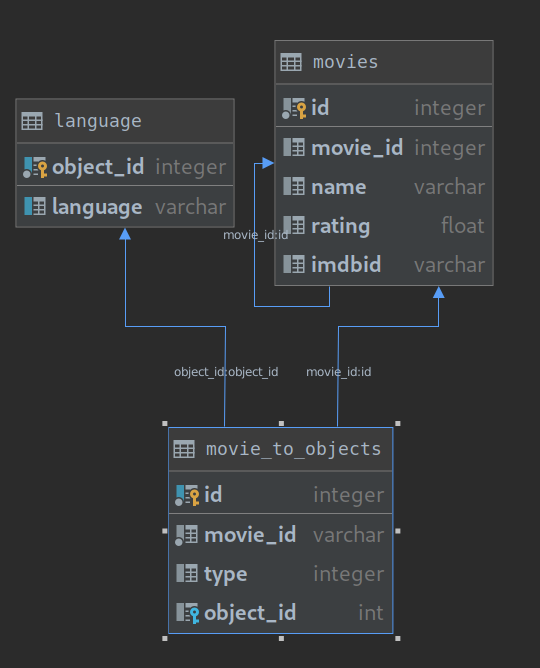
\includegraphics[scale=0.25]{dbLink2.png}
                        \end{center}
                        \caption{Database Implementation}
                        \label{fig:dbLink2}
                    \end{figure}
                    

                We also had to move to use the SQLite3 module as although using SQLAlchemy meant we had easy to use Python objects. Creating a Python object for every line in a table is a slow way of adding things to a database and would be too slow to continue with. The API that was explained in \ref{sec:CollectingMovies} returns a number of pieces of metadata. We turned some of these into explanations. Below is a list of items that can be used as explanations:
                \begin{itemize}
                    \item Actor
                    \item year 
                    \item director
                    \item genre 
                    \item rated (The MPAA rating system)
                    \item released (Year of release)
                    \item runtime 
                    \item writer 
                    \item language 
                    \item awards (Any awards the movie has won)
                    \item productions (The production studio that made the movie)
                    \item country
                \end{itemize}
        
                The code shown below in figure \ref{fig:CreatingExplanations} shows how the system takes objects from the \textit{movie\_to\_objects} table and creates results that we can use in creating explanations for each user. This needs to be done for each movie that is being recommended. This returns the result from the SQL query which is then used to make an explanation object for each item returned. When creating them they are scored based on the number of times they appear in your profile or random depending on whats needed. When creating the debate the explanations with the highest score are picked. They are given a score between 0 and 1. In figure \ref{fig:ScoringExplanations} we show how some of the explanations are scored. As part of creating the explanation objects they have a number of methods that are used in their creation. It was decided that using the SQLite3 module instead of using the SQLAlchemy would work better because the below statement would have been much harder to create using SQLAlchemy. Each object in the database which is a piece of movie metadata is represented by an object id and a type. Each type has its list of objects. For example actor Tom Hanks has object id 792 and is of type one. We have an enum representing the different objects that exist so they can easily be referenced.
                
                
                    \begin{minipage}{\linewidth}
                    \begin{lstlisting}[gobble=20, tabsize=4, caption=Code used to retrieve data for explanations,label=fig:CreatingExplanations]
                    def compare_movie(IMDB_id, user_id):
                        c,conn = get_db()
                        query = """
                        SELECT  t1.type, t1.object_id , COUNT(*)FROM (
                        (SELECT movie_id,type,object_id FROM movie_to_objects
                        WHERE movie_id == ?) t1
                        LEFT JOIN
                        (SELECT movie_id, type, object_id FROM movie_to_objects  GROUP BY
                        object_id, type , movie_id HAVING movie_id in (SELECT IMDB_id FROM
                        movie_id_to_IMDB_id
                        WHERE IMDB_id in (SELECT user_ratings.IMDB_id FROM user_ratings WHERE
                        user_id == ?))
                        ) t2 on t1.object_id = t2.object_id AND t1.type = t2.type) GROUP BY
                        t1.type, t1.object_id ORDER BY t1.type;
                        """

                        c.execute(query, (str(IMDB_id), int(user_id)))
                        result = c.fetchall()
                    \end{lstlisting}
                \end{minipage}

                    \begin{minipage}{\linewidth}
                        \begin{lstlisting}[gobble=24, tabsize=4,  caption=Code used to rate an explanation, label=fig:ScoringExplanations]
                            def get_score_for_type(self):
                                max_for_type = get_max_for_type(self.explanation_type)
                                min_for_type = get_min_for_type(self.explanation_type)
                                normal = (self.count - min_for_type) / (max_for_type - min_for_type)
                                return normal
                        \end{lstlisting}
                    \end{minipage}

                As an alternative to the above explanations we did create some more examples of explanations but they did not get used in the system that we built. An example of this is shown in figure \ref{fig:past_performance}. This method takes a movie as input and will return the average rating of the movies the director has directed. It ended up not working with the system that we implemented but it could have been worked on in the future.


                    \begin{lstlisting}[gobble=20, tabsize=4,  caption=Code used to get the past performance of the movies of a director,label=fig:past_performance]
                        def past_performance(movie_id):
                            query_for_director = """
                            SELECT SUM(rating)/COUNT(rating) FROM movies_2 WHERE IMDB_id in (
                            SELECT movie_id from movie_to_objects WHERE \
                            object_id == (SELECT object_id from
                            movie_to_objects WHERE movie_id == ? AND type == \
                            3) AND type == 3);"""
                            
                            c.execute(query_for_director, (movie_id,))
                            response = c.fetchone()
                            if response is not None:
                                return response[0]
                            else:
                                return None
                    \end{lstlisting}

            \subsubsection{User Interaction}

                The first two systems were only usable on the command line where you would supply parameters and it would give you back information. As we wanted to create a whole debate system with user trials we needed something more interactive. We decided on a website using Flask. Flask is a micro web framework that can be used with Python. We had previous experience with it from a group project so it seemed like a good choice. There are other similar options out there like Bottle. Flask does not require you to use certain tools with it. You can use whatever you like. We will talk about reasons we picked Flask more in a later section \ref{sec:webDevelopment}
                
                As part of the requirements, we needed the user to be able to input information such as movie ratings. We created four main pages. 
                The showings page was used for testing before we created the debate. This page shows the current movies for a user and all of the explanations for those movies. The ranking page contained the controls for the debate and user trials and gave the user the ability to add ratings to movies in the system. When the user gave a rating we would get the data that was returned from the Flask form and we used the function \textit{rate\_movie(user\_id, IMDB\_id, rating)} to update the \textit{user\_ratings} table with the new information. This either involved finding the existing rating for that movie or creating a new row with the IMDB id and the rating. We also have a page that would let a user take an IMDB id of a movie they wanted to rate and it would import the information about the movie into the system like explained in section \ref{sec:CollectingMovies} 
                
                The controls of the debate and user trials could be used to create a new debate, start a new user trial or reset an already existing one. The last page we had was the debate page. This would be used after a user had created a debate. It would show a set of movies and their explanations and would update at the end of each round of the debate. The debate page like other pages had the nav bar at the top, along with the six posters for movies we would be recommending and their explanations. Below that we had a selection box that allowed the user to remove a movie.

                Initially the plan was for a user to rate movies and then create a debate which could be stored in a JSON format to be used later. When the user created the debate, it would pick a set of movies as explained above and it would create explanations. The system would then store the JSON using the function \textit{write\_to\_json}. This would accept a JSON dictionary and write it to a file to be accessed later. When the user accessed the page for the debate we would then retrieve the debate using this file and show it to the user. At the end of each round, the JSON would be updated by removing the chose movie along with its explanations. 

                Instead of continuing to store the program's state in JSON we moved to using the database. This was necessary as we started to work on Implementing the user trials. We would need to keep track of what round each user was on and their debate. When the user creates a debate we store the movies that were selected in the database along with the explanations for those movies. This involved creating a new table to store created explanations for each movie and a table for the movies the user was to be recommended. The explanations were stored in the form:

                \begin{itemize}
                    \item id (the distinct explanation id for the database)
                    \item user id (the id of the user who created the debate)
                    \item IMDB id (the movie id the explanation related to)
                    \item count (the number of times the object appeared in the user's profile)
                    \item type  (the type of object this was e.g. actor or director)
                    \item object id (id of the object in its respective database table)
                    \item explanation string (the explanation given to the user in the debate)
                    \item rating (the rating the explanation was worth)
                \end{itemize}
                
                The soon to be recommended movies for a user were stored with:
                \begin{itemize}
                    \item id (the distinct id of the relationship between this movie and the user)
                    \item user id 
                    \item IMDB id 
                    \item movie title
                    \item poster filename (where the poster is stored in the system)
                    
                \end{itemize}

                These two tables can be pulled from to form the debate. When the users goes to the debate page the system finds the current movies they are to be shown for that user. The round of the debate and the user trial was also stored in the database for each user. Based on the round of the debate the system picks explanations for each movie. The debates start with one explanation per movie and each round adds one for each movie. At the end of each round the user removes a movie this movie is then removed from the \textit{current\_movies} table for the user so it will not be included in the next round. 
                
                The user trial has six rounds which are split in half. Each debate in the user trials has different modifications applied to it. The round of the user trial is checked when creating the debate. This is then used to determine three settings. The first is which movies to recommend either, movies from the cinema or movies from the Pearson calculations. This setting is inactive for the first three rounds but is activated for the last three. The setting being inactive means we take movies from the local cinema and active means we take movies from the Pearson calculations. The second is whether the user sees a poster and movie title with the explanation. The final setting is whether the explanations are created with our custom scoring function specific to the explanation type or assign a random score to each explanation. We had a function \textit{return\_settings} that would return a triple of settings based on the user trial round. As part of moving the debate and user trials we created a suite of methods that would manage the inserting updating and removing of debates and user trials from the database.
                
                
        
                \subsubsection{Presentation}\label{sec:webDevelopment}


                    As we mentioned above we are using Flask to create the website. Flask routes allow you to map urls onto Python functions. When a url is visited the function matching that is run. For example our system has a route for any GET or POST requests that come to \textit{/user/<username>/debate/} will run the \textit{debate\_page()} function. In this function, we can call other functions to create a page and then at the end we can use \textit{render\_template()} to return content that will be used in the Jinja template.

                    Jinja is a web template engine designed to be used with Python. it uses text-based Python like expressions. Its the default template engine for Flask and it integrates well with it. it allows us to define templates for pages programmatically without writing HTML. It also integrates well with Flask forms which only requires on line to create and show the forms on the page. It also allows the use of base templates that can be included in other which reduces the reuse of code between pages. Base templates are extended to create the new template. These are useful for containing style sheet links and navigation bar html\ref{fig:JinjaTemplate}
                

                    \begin{lstlisting}[gobble=20, tabsize=4,  caption=Jinja template example, label=fig:JinjaTemplate]
    
                        
                        
                    
                        
                        <h1>{{ _('Rank movies') }}</h1>
                        <div class="col-md-4">
                            {{ wtf.quick_form(form) }}
                        </div>
                        
                        \end{lstlisting}

                    One of the reasons we tested out using SQLAlchemy was because there is a version called Flask-SQLAlchemy that can be used with Flask. It also supports the use of WTForms which is a library for quickly creating web forms. Flask lets us easily create pages for the project. We can define the location of the page using the code shown in \ref{fig:CodeToCreatePage}


                    \begin{lstlisting}[gobble=20, tabsize=4,  caption=Code to create page, label=fig:CodeToCreatePage]
                        @app.route('/user/<username>/rank/', methods=['GET', 'POST'])
                        @login_required
                            def rank(username):
                                form = debateForm()
                                return render_template('recommender/rank.html', user=username, form=form)
                    \end{lstlisting}

                    In the page function we can retrieve what is going to be shown on the page for the user and then pass that as parameters of the function. In this page we are using a Flask form that accepts the user rating for a movie. In the debate page a JSON object is created that contains the movie title, poster and the explanations. This is returned in the render template function. The jinja template created for the debate page then parses the JSON and shows the movie and explanations. To update the debate each round we can just change what gets passed into the jinja template. 

                    
                    One of Flask's best features is the ability to create a development web server that can be used for rapid prototyping. When using the production Flask web server, it has to be restarted every time a change is made in the code for it to be represented in the system. This makes sense for production where you would not like your web sever to restart suddenly when a developer makes a change. On the other hand the development server will automatically restart when it detects a change in the code which speeds up development as it takes much less time to make a change and see it represented. This also integrates with Visual Studio Code's development workflow and the debugger in can be setup to walk through the code and add breakpoints to inspect variables as the code is run. This is incredibly useful during development. When finished developing and moving the website to production it is advised to move away from using the built-in web server and instead use a production-ready one.

                    Another advantage of Flask is its ease of use. When developing we used \textit{Flask-Bootstrap} for the look and feel of the website. This is an extensions that consists mostly of a Flask blueprint that makes it easy to use the Bootstrap front end library with the project. It automatically applies a default CSS to the website when included. This was enough for us as the appearance of the application was not what we were going to spending time on. When we started to do user testing we realised that because we used Flask and Bootstrap the website worked perfectly when used on mobile devices. Flask Blueprints allow a developer to separate their code into modules. This is great for a large project. We had a separate blueprint for our login system. We were able to separate that code out into its own folder where we could create a set of routes that are accessed from the main application. They can be accessed from the main application once they are registered. 
                    
                    Gunicorn is a Python Web Server Gateway Interface HTTP Server. It is built to have many different web service interact with it as long as they use this gateway interface. The WSGI is a way to make sure that web servers and Python web applications can easily talk to each other. The web application can be created by Gunicorn and used to handle more requests. There is an alternative to Gunicorn called uWSGI that does a similar job. We did not have many static pages in our application so we did not use a web server. Nginx is an example of one of these. We would not be serving many people or static pages so it was not required that we use one. This would be inefficient for a larger scale application as Nginx is developed to serve more users and static pages at the same time which is helpful. This web server would stand between the Flask application and Nginx.

                    Docker is a containerization platform that allows developers to isolate their application from its environment. It lets the developer package the application and all of its dependencies into one container. This allows us to redeploy the application easily to different places that support Docker containers. Which is any Linux Server with the docker software installed. They use OS-level virtualization to host applications. This means all docker containers on a host run on the one operating system reducing the amount of computation needed compare to a standard virtual machine. 
                    
                    Initially we used a single Dockerfile to contain all the configuration for our application but we moved to using Docker Compose instead as it allows us to integrate with Traefik which would reroute our web traffic to the application running on the server. This routes traffic received on ports 80 or 443 to a specific docker container based on the url specified. This is useful if you are running multiple services on one machine which docker supports. 

                    A domain was purchased to be used with the application. Using Cloudflare DNS this let us point the domain at the static IP address of the server. Any Traefik bound for our application would then be checked by Cloudflare for malicious intent before it reached the web server. After it had routed through Cloudflare and it reached the server it would be sent to Traefik which would take any traffic for http://recommender.domain.xyz it will route that traffic to the docker container running the Gunicorn server hosting our application. 


                    \subsubsection{Critique}
                        Implementing the storage of the explanations in a JSON file seemed fine at the time but expanding it out for use with the debate was over complicating the program. It would have been better to move to using a database to store the state of all of the application's states earlier in the project.
                        As we will mention in the evaluation chapter \ref{sec:userTrials}, there were some bugs in the system that could have been fixed with a better testing plan. Even though the database is more extensible that the methods we used in previous systems there are still ways to improve it such as making it more generic to the type of data being used. 



            \subsubsection{Data Flow Diagram}
            \begin{figure}
                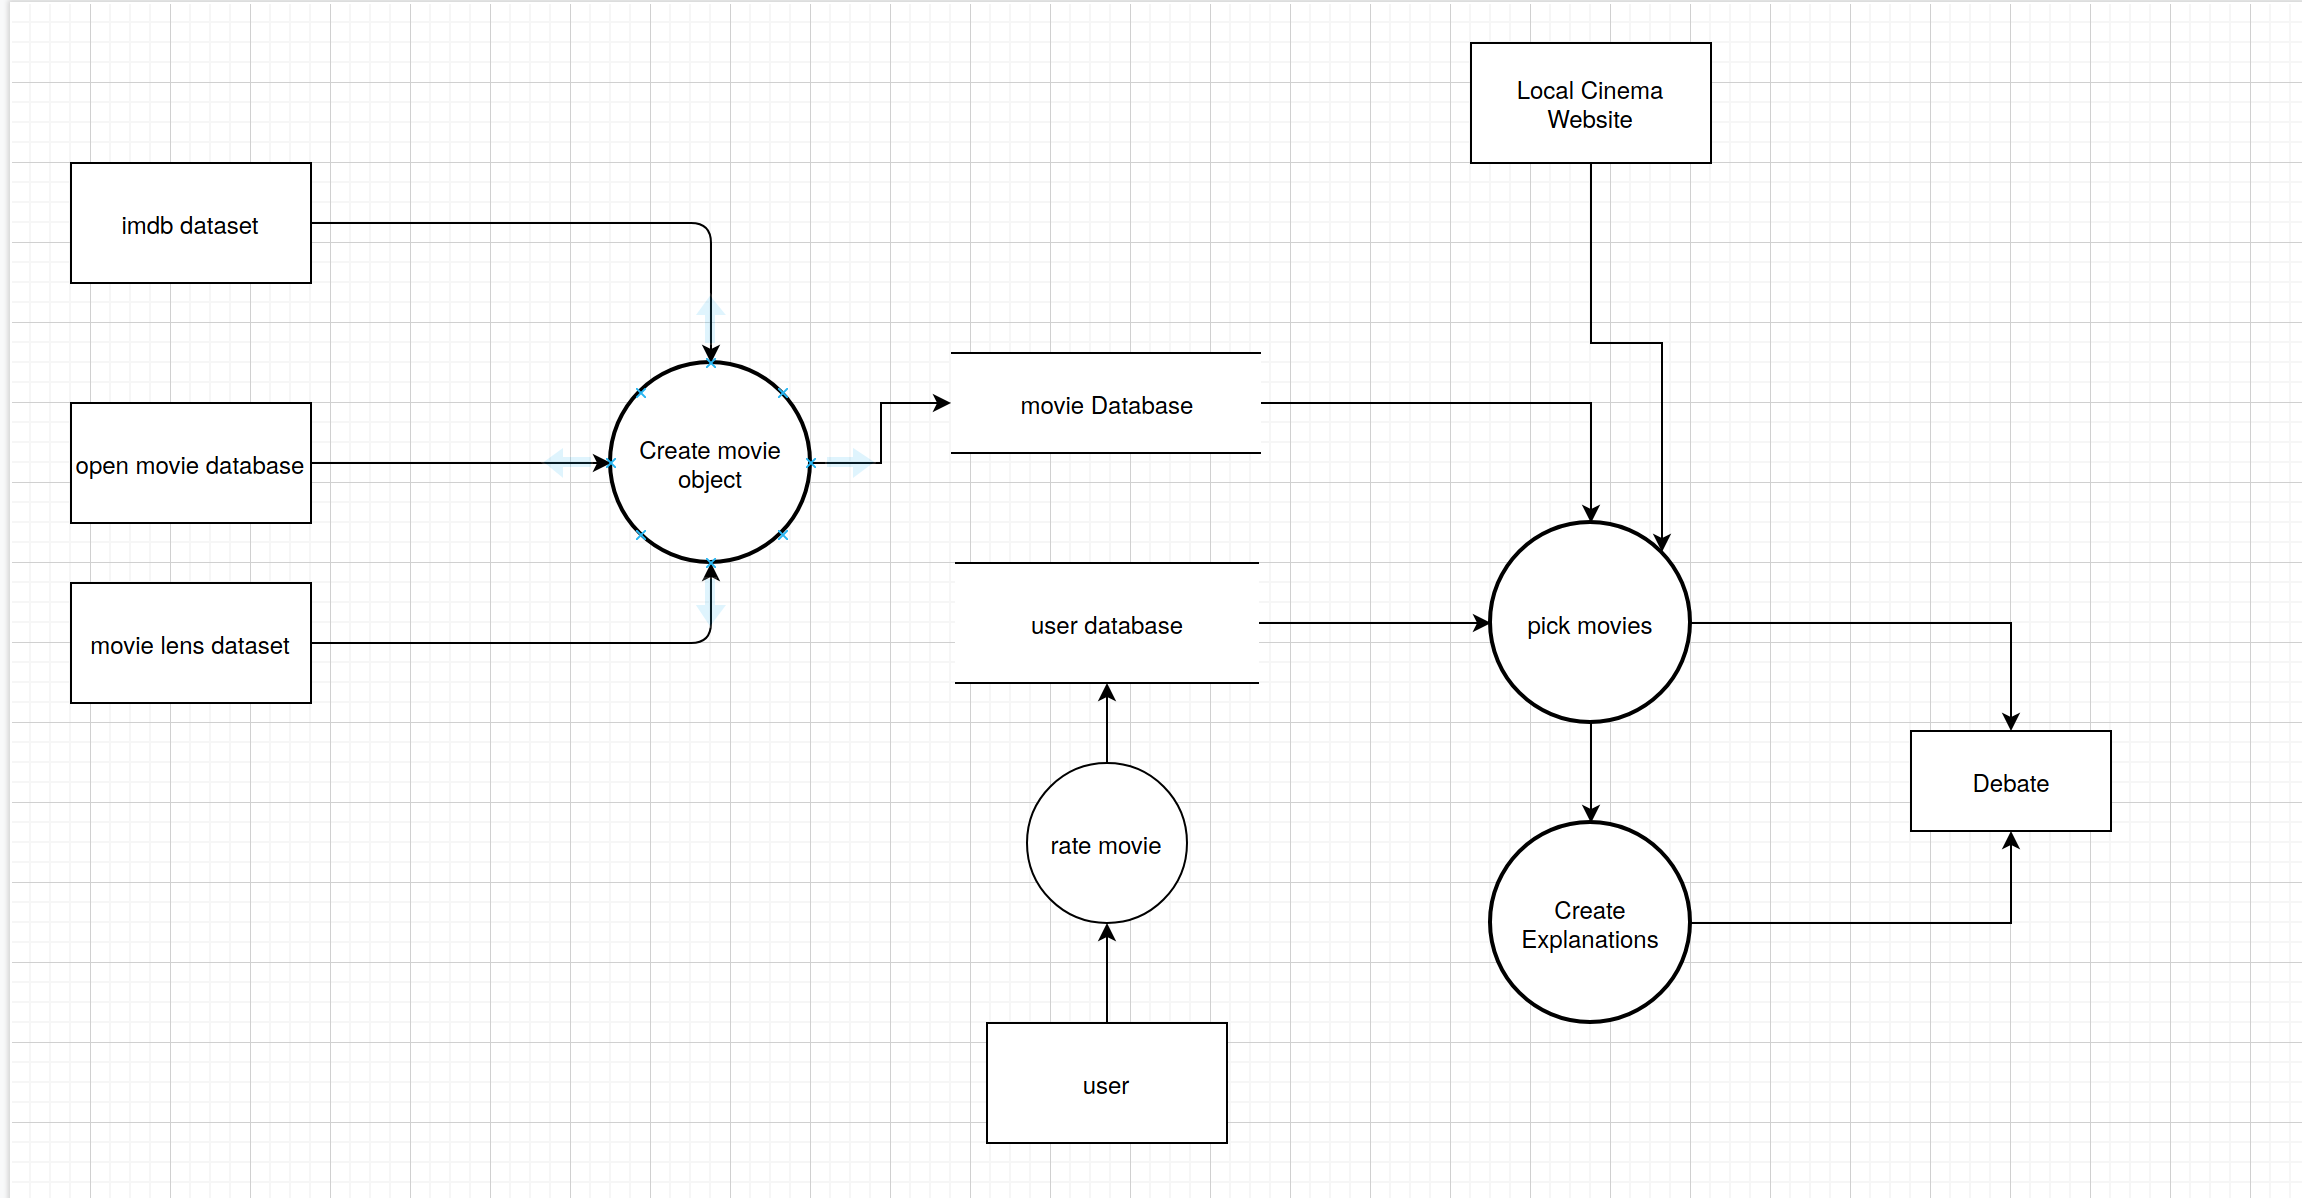
\includegraphics[width=100mm]{DataFlowDiagram.png}
                \caption{Data Flow Diagram}
                \label{fig:DataFlowDiagram}
            \end{figure}
            
            As shown in figure \ref{fig:DataFlowDiagram} the data comes in from the open movies database and gets turned into database objects. User ratings from the movie lens dataset gets put into the users\_ratings table. when creating the debate the movie titles that are going to be recommended get taken from either the user database in the case of movies recommended by neighbour or from the local cinema. These are then used with the movie objects database to compare movies. Explanations are created this data and shown to users in the debate. 


            \subsection{Example}
                In our final system we are able to give the id of a movie into our system and it will get all the objects that are related to that movie and cache them. For example let us look at the movie Iron Man (2008) which is represented by the IMDB id \textit{tt0371746}. It will first get passed to the function \textit{scrape\_omdb\_with\_movie\_id(imdb\_id)}  which will take in an IMDB id which are of the form tt then seven or eight numbers. This function will consume the JSON response from the OMDB API shown in Appendix \ref{fig:ironmanjson}. This is then passed to the function \textit{filter\_movie(response)} which looks at each section of the JSON, extracts it, checks if it's in the database already and if not creates it. It then creates a link between the object and the movie. 
                
                Each section in the JSON is a type which is represented by a number from an Enum which makes it easy to reference. The resulting database additions look like what is show in \ref{fig:ironManObjects} Each line in the database represents an object be it an actor or the production company. Each type then has its own table that has the same object id with a string for actor names or a string for the poster link etc.



                % \begin{figure}[!htb]
                %     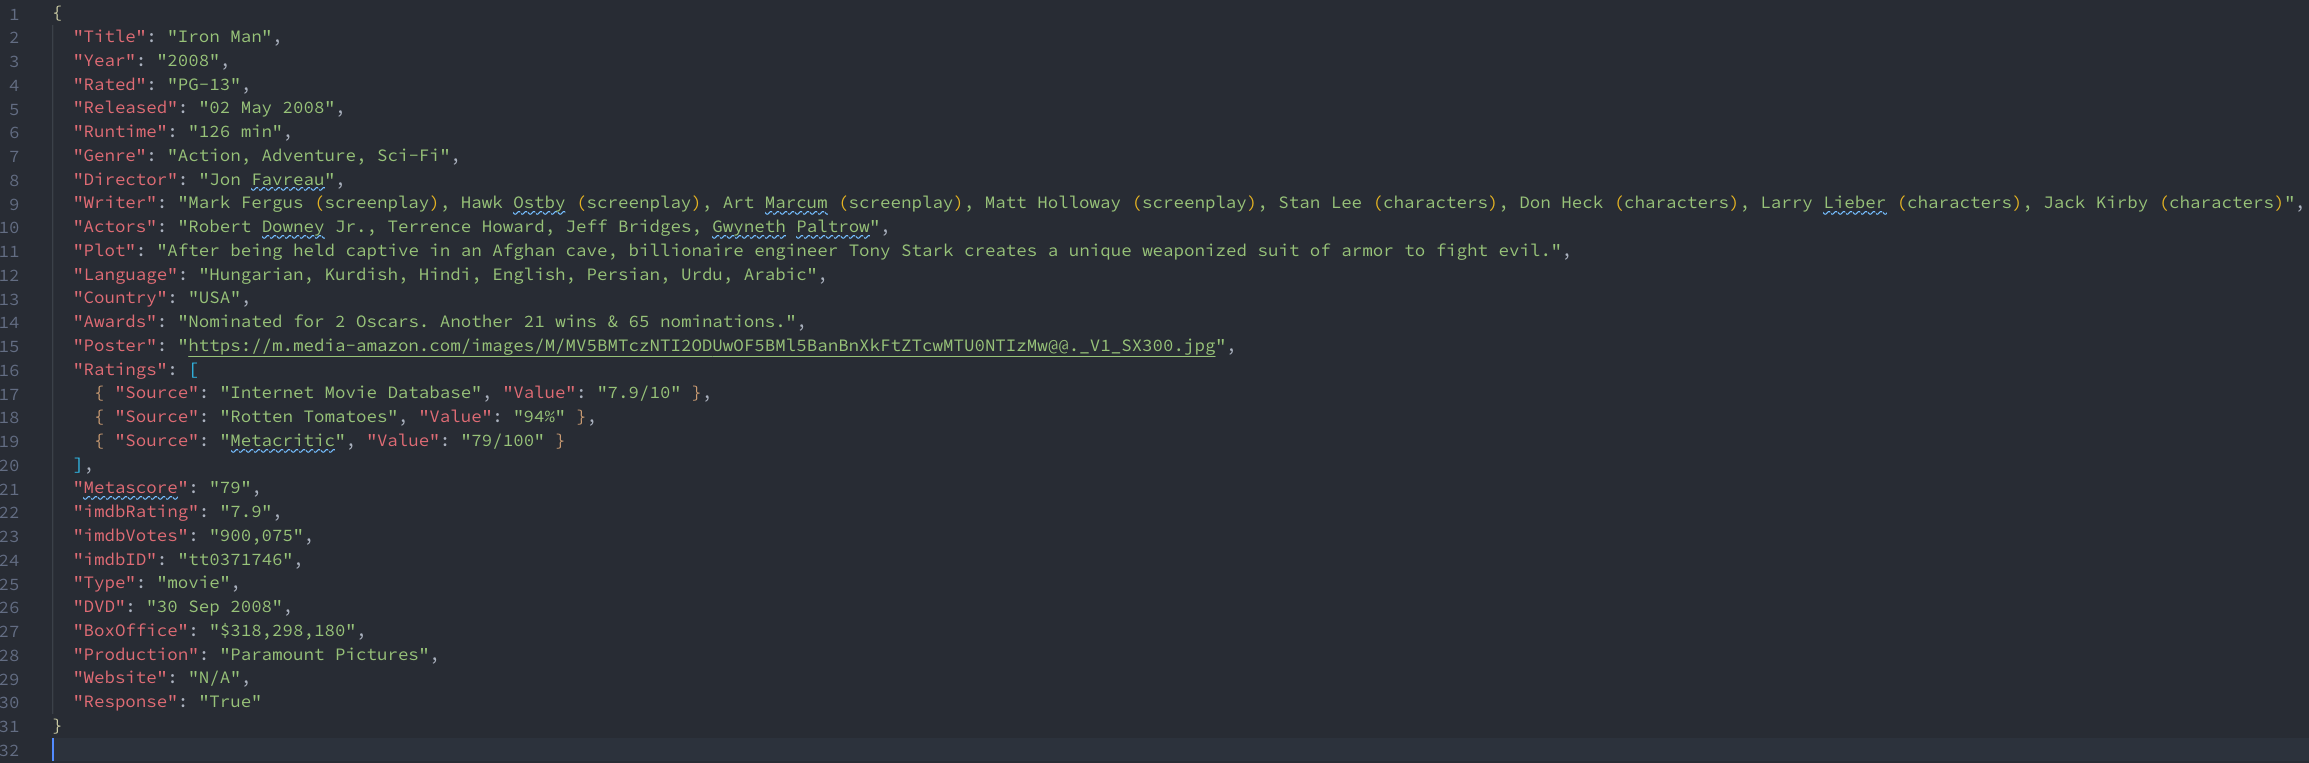
\includegraphics[width=100mm]{ironManJson.png}
                %     \caption{JSON returned for Iron Man}
                %     \label{fig:ironmanjson}
                % \end{figure}

        

                \begin{figure}[!htb]
                    \includegraphics[scale=0.25]{ironManObjects.png} 
                    \caption{Objects created by the importer for the movie Iron Man 2008}
                    \label{fig:ironManObjects}
                \end{figure}



                After each object has been created and stored, we can use the code in figure \ref{fig:CreatingExplanations} with a user id and the iron man movie id. This will give us the common objects between the user's profile and the movie. This is shown in figure \ref{fig:ironManObjectsCount}


                \begin{figure}[!htb]
                    \includegraphics[scale=0.25]{ironManObjectsCount.png} 
                    \caption{Common objects between the user with id 611 and the movie Iron Man (2008)}
                    \label{fig:ironManObjectsCount}
                \end{figure}


                After these have been created, each one gets turned into an explanation. The information is stored in a Python object along with a string that can be printed out to the screen and a score for that object related to its count. 

                The system then takes each one of these explanations and ranks them by score and uses the best in the debate. When the user begins the debate the movie is shown on the screen and we can see the explanation underneath. In figure \ref{fig:ironManSelection} we show the explanations that would be given if iron Man had won with its six explanations. The explanations are shown ordered by decreasing the score. 

                \begin{figure}[!htb]
                    \includegraphics[scale=0.4]{ironManSelection.png} 
                    \caption{The explanations produced by the system and shown with the movie Iron Man (2008)}
                    \label{fig:ironManSelection}
                \end{figure}

                We also had the ability to create explanations and score them with a random function. This produced the debate show in figure \ref{fig:ironManSelectionRandom}.

                \begin{figure}[!htb]
                    \includegraphics[scale=0.4]{ironManSelectionRandom.png} 
                    \caption{The randomly scored explanations shown with the movie Iron Man (2008)}
                    \label{fig:ironManSelectionRandom}
                \end{figure}

            
            \subsection{Critique}
                The focus of this system was to get it working so that a user could participate in the debate. In some of the rounds, we do not show the title or the poster of the movie. This can lead to some confusion as we have to refer to the movies from the selection box. A better way to do  this would be to place a button near each movie that would let you remove that one. The scoring of the explanations can sometimes lead to items that are not the best explanations being used. A better algorithm could have been created to calculate the usefulness of an explanation.


   
\chapter{Evaluation \& Experiments}\label{sec:userTrials} % 6 pages
    
    In this chapter, we are going to discuss the user trials that were conducted at the end of the experiment and the results that were taken from these.

    \section{User Trials}
        Originally we were going to do user testing in person with the prospective users. This was to ensure that no problems would be encountered and that we could explain the steps in person before they started the testing. This was not possible as the project was not completely ready to be tested before the college shut down because of COVID-19. Instead, we created a suite of questions to ask users after they had completed using the recommender. In \ref{sec:UserTrialQuestions} we will explain the questions and the reasons behind them. As explained in section \ref{chap03-sec:3UserInteractionDesign} we designed a page to manage the use of the user trials so they can be conducted by the user by themselves. 

        Now that we were doing the user testing online we started with a small group of initial testers. This was used to iron out any bugs and to see if the questions were appropriate. When the application was set up for the user to begin testing we identified a few bugs. One of them was when explanations were being created there was a bug where the server would time out as they took too long to generate for one round. This was related to the number of movies in one's account and was fixed by changing the web server used. One type of explanation when created was using corrupt data. The API returned a not applicable string and this was entered into the database and used to create an explanation. This data was removed from the system to solve the error. Following this, we asked a number of people to use the system over the six rounds and to answer some questions at the end.

    
        \subsection{User Trial Questions}\label{sec:UserTrialQuestions}
        
            \begin{enumerate}
                \item In round 1 and 4 there were no titles or posters did this affect your choosing of a movie? if yes how important on a scale of 1-5 would you say posters and titles are?
                \item Did you notice anything different about the explanations in round 3 and 6 compared to other rounds?
                \item rounds 1,2,3 and rounds 4,5,6 had different movies. Did you notice a difference? was there a set that was better?
                \item On a scale of 1-5 would you find a system like this helpful?
                \item On a scale of 1-5 did you find this more interesting than a normal recommender?
                \item did you see any explanation types that were particularly interesting?
            \end{enumerate}

            We created these questions to evaluate the system that we had created. We wanted to find out what people thought about the system and whether it was a worthwhile use of their time. In question one we were referring to rounds one and four which were the first rounds using the different sets of movies. In these rounds, we did not show the user the movie titles or posters. They were only given the explanations we created. This was a test to see if the explanations we created contributed to a user picking a movie or if they were going to base it on the title and poster. We are hoping to see that most users found an explanation they liked and it was not just the best poster.
            In question two we asked whether users noticed a difference in rounds three and six. In these rounds, we changed the scoring system for the explanations to use random scoring where each explanation is given a random score. This was to test if people found explanations score with our scoring system more useful than random. There is a possibility that random will give some good results sometimes. 

            In question three we are asking the user if they noticed anything different about the sets of movies in the first three rounds vs the last rounds. The first three rounds take movies from the local cinema which should mean the user is  less likely to like the first set. The second set of movies were based on what a user's neighbours have rated highly. The original aim of the project was to use movies from the local cinema in the system. We wanted another set of movies to include so we used ones recommended by a user's neighbours.

            Question four and five were asked to see if the user found the system helpful or more interesting than a normal recommender they had used before. Hopefully, we will see that users have found the system helpful or even an interesting way of getting movie recommendations. 
            The final question was asked to see if any of the explanations in particular resonated with a user. This will probably be highly dependent on the person's tastes. The questions were sent out with some instructions on how to use the system to a group of people. 
         
        
       \subsection{Responses}

            
            \subsubsection{Question 1}
                we can see from the results of question 1 people think the movie poster and title are important in choosing a movie.This seems like an obvious conclusion since movies are inherently a visual medium. When someone is looking at a movie poster they get information about the movies such as the genre or style of the cinematography. They may also be able to recognise any actors that are in the movie. Neustar on behalf of Facebook evaluated 70 major studios across a variety of genres. These studios spent more than 1.8 billion on marketing in 2016. Over 80\% of this was on TV advertising. For example Avengers Endgame which was released in 2019 its budget was 356 million dollars. Another 200 million was spent just to advertise the movie. This movie grossed 2.8 billion dollars by the time it was finished showing around the world so money well spent. People seemed to regard the poster important. Although a few responses indicated that a neighbor's rating mattered more than the poster and title. As we can see from the results from question 1 in \ref{fig:Question1Results} people feel the poster and title are important.


                \begin{figure}
                    \centering
                    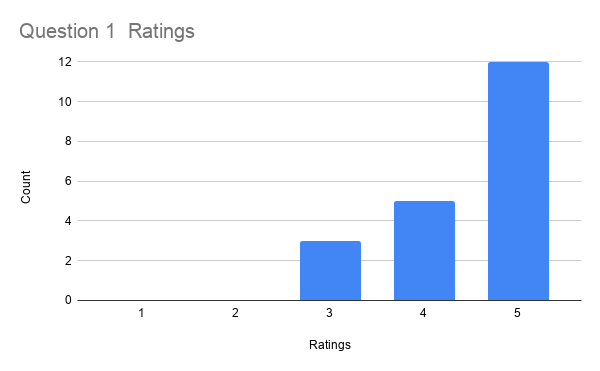
\includegraphics[width=100mm]{Question1Results.png}
                    \caption{Results from Question 1}
                    \label{fig:Question1Results}
                \end{figure}


            \subsubsection{Question 2}

                The second question was related to which scoring system was currently being used. In round one, two , four and five we were using a custom scoring for the explanations. In the third and final rounds, we were using random explanations. This was designed to test if our scoring function made people think differently about the explanations that were created. Our custom scoring system was based on the number of examples of an object that were in the system compared to the number of times that object appeared in the system in total. We would expect people to like the custom scoring method more as it applies to movies they have seen before. Although the random scoring might rate an explanation that resonates with someone more and could create some serendipity. In the random selection of explanations, it seemed to pick the actor and director more than other attributes. In the scored explanations  other than actor and director seemed to get picked. Some people preferred seeing actors and directors. This would leave me to believe the scoring function for some explanations needs to be tuned to how helpful explanation has been in the past to someone. 

            \subsubsection{Question 3}
                The third question pertains to the difference between the movies we used in rounds one to three and four to six. In rounds one to three we used movies from the local cinema and in rounds four to six we used movies we were recommending based on a user's profile. The first three movies were taken from the cinema's website and certain The most recent six movies that were released were picked. This would mean the movie selection will get changed out fairly often as new movies are released. Through the year movies might not make it into the system as sometimes the number of movies released per week is more than the system can show so only some are picked. The cinema updates its movie selection every Thursday. There might be times during the year where none of the new movies that are released matches a user's taste so in that case movies based on their profile are much more likely to be picked. As we can see in \ref{fig:Question3Results} the majority of users picked the 2nd set as the movies they preferred. Some seemed to like the movies that were new as well. 


                \begin{figure}
                    \centering
                    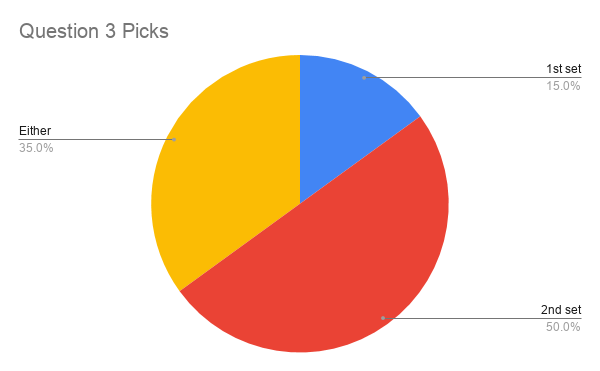
\includegraphics[width=100mm]{Question3Results.png}
                    \caption{Results from Question 3}
                    \label{fig:Question3Results}
                \end{figure}



            \subsubsection{Question 4}

                The fourth question was asked to find out if people thought the system was helpful compared to a normal recommender they may have experienced before. As we can see most users rated it at a four out of five in terms of helpfulness to them. As part of this question, we asked the users to respond with why they found it helpful. We did not pick a recommender that they should compare it too as we are assuming most are familiar with Netflix or a similar movie streaming website even if they are not intimately familiar with how the system works they have has movies recommended to them before. As we can see in figure \ref{fig:Question4Results} the most popular rating was four out of five. Based on feedback provided as well as the results, people found the system helpful but hampered by the fact they had to input movie scores before using the system. and were not greatly fond of having to complete an entire debate to get explanations. This could be just passively given to a user while searching through a streaming service. 

                \begin{figure}
                    \centering
                    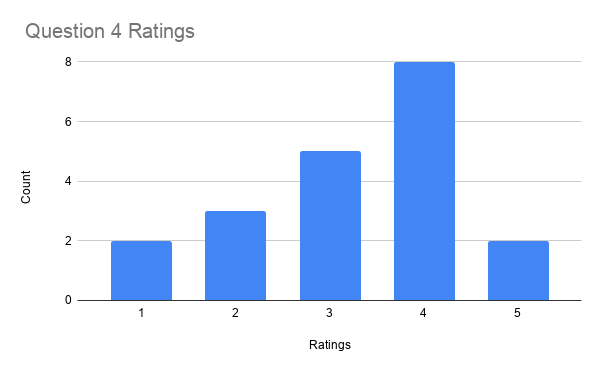
\includegraphics[width=100mm]{Question4Results.png}
                    \caption{Results from Question 4}
                    \label{fig:Question4Results}
                \end{figure}


            \subsubsection{Question 5}
                The fifth question related to whether users found the recommender more interesting to use than a normal recommender. Part of the goal of this recommender was that it would create interesting recommendations. Similar to the last question users felt the system was interesting. Most of the users who tested the system rated it at four out of five \ref{fig:Question5Results}. People found this fun to play with and more interesting that just being shown the movie they might like. 

                \begin{figure}
                    \centering
                    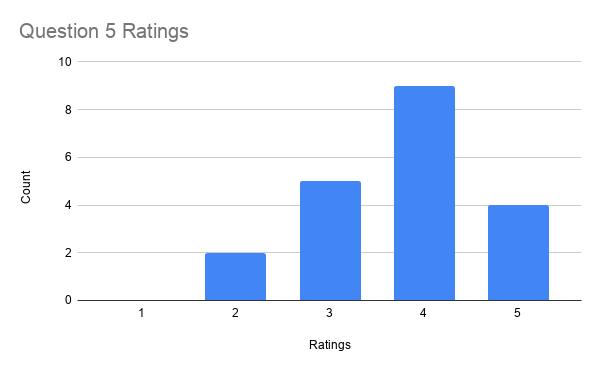
\includegraphics[width=100mm]{Question5Results.png}
                    \caption{Results from Question 5}
                    \label{fig:Question5Results}
                \end{figure}


            \subsubsection{Question 6}
                The last question we asked to find out were any of the explanations particularly interesting to the users. Again this is a subjective question but was mainly to see if users found any particular explanations were helpful while picking a movie. This seemed to vary quite a lot between users as it's up to their tastes. Many liked the information about actors and directors especially if they were aware of who they were. There were also a few votes in favour of genre.
                It would be interesting to implement this into the scoring system based on what movies people removed and increase the weight given to explanations that swung the debate.
        


        \subsection{Conclusions}
            We have seen that most people found the system interesting and it created some explanations that people found helpful and interesting. After completing the user trials we had removed some bugs from the system and gleamed more information about how users feel about the system and how they would use it in practice. This has been very worthwhile and gave us more information about what we can improve about the system in the future. We will explain this in section \ref{sec:FutureWorks}
\chapter{Conclusions \& Future Work} % 3 pages
    In this chapter we are going to discuss the conclusion reached with the project and we are going to discuss some future work that could be completed given different circumstances. 

    \section{Conclusion}
        Our goal was to create a system that would facilitate a debate between movies thereby helping a patron to make a movie choice. This was achieved in that movies created explanations that the user found helpful in refining their choice. The results from the questionnaire shown above demonstrate the achievement of this goal. 

    \section{Review of Requirements}
        As part of designing the system a number of functional and non-functional requirements were laid out before we started work on the project in order to ensure there was a clear structure to the project. These were laid out in section ~\ref{chap02-sec:Requirements}. In this section, we are going to describe what was expected and what was completed. 


        \subsection{Function Requirements}
        \begin{itemize}

            \item The user must be able to search and rate movies to add to their profile.\\
                Two pages have been created to do this. The first has a list of movies in the system and a user can apply a rating to any of these movies. If they have already rated a movie they can re-rate the movie. On the other page the user can add a movie to the system by its IMDB id tag or its title and add a rating there. 
            \item The user must be able to take part in user trials which accommodate a number of debates.\\
            The debate-page was created for a user to take part in the debate created for them. This page shows movie information pulled from the database along with the created explanations. 
            
            \item The user must be able to view the movies attached to their profile.\\
            This was completed as part of the back end of the application but a page was not created to show this to the user. 
            \item The user must be able to view other users and the movies on their profile. 
            \end{itemize}
            A user is able to see other users but they are unable to see the movies in their profile. Like above this can be done but is not shown on the front end. 
        \subsection{Non-Functional requirements}
            \begin{itemize}
            \item The user should be able to view explanations for recommendations.\\
                In the second system this was done through the use of the show movies page which showed local movies without the debate structure. This just listed each movie from the cinema and then all the explanations created for that page. Then in the third system this was rolled into the debate page. Depending on the round of the debate a number of explanations were shown in addition to the movie information provided. 

            \item There must be a frontend for a user to interact with and there must be a single source where the data is stored.\\
                As part of the third system a simple web app was created for a user to interact with. This was made up of only a few pages that were necessary for operation. 
            \item The state of the user testing and the debates should be stored during operation.\\
                A user's state in the debate and user trials are kept throughout their use of the website. The status can be reset also
            \item The user must be able to add their own ratings to the system.
            \item The movies should create explanations for themselves. 
                \begin{itemize}
                    \item These may be scored relative to other explanations\\
                    During the course of the user trials each round has different settings that are turned on and off. On of these settings it the ability to change the scoring function of the explanations between random and a scoring function based on the popularity of the item. This fulfills both requirements.
                    \item Or they may be scored randomly for serendipity.
                \end{itemize}

            \item The system must be able to import information about new movies as they come out.\\
            In the first system, we were only using the current ratings from the Movie Lens dataset. 
            \item The system should be able to compute the Pearson correlation between movies and users. 
            \end{itemize}

        As we can see above almost all of the functional and non-functional requirements were satisfied.
        Before the start of the user trial,s there were a few things we were unable to finish. One was the ability for movies to pick a bad explanation from one movie and use it as their own. We planned for a movie to take an explanation that might have been negative about a movie and use it to dissuade a person from picking the movie. Another was the ability for a user to see movies they had in their profile. The second would require a simple page that finds movies a user has rated from the database and presents them on a page. We already get all the movies they have rated when creating an explanation. This was an overlooked feature what would have been helpful during user trials. The final system was unable to have movies compete against each other using negative explanations for one another but were able to use positive explanations for themselves. This was a planned feature but as time got closer to user testing and with the move to having to implement a system to have users be able to complete the system trials online this was not completed. As all of the explanations that are created are given a score. It would be a fairly simple extension to allow a movie to pick a negatively rated explanation from another movie and use it against the movie the explanation was created for. After completing the user trials and looking back at the original requirements there were a number of things we could work on in the future. This leads us into the next section where will talk about the parts of the project that could be undertaken in the future.
        
         
    
    \section{Future Work}\label{sec:FutureWorks}
        As we talking about at the end of the user trials a lot was learned from the responses. In this section, we are going to mention some of the ways the system could be changed to improve the user's experience with the system and to improve the system in general. 
        

        \subsection{Expandability}
            During the project, we attempted to make the system as expandable as possible. The system was created to make it easy to add more explanations to it. The same SQL can be used as long as more explanations are added in the same ways as they currently are. Originally all explanations were created from the database of objects but towards the end, we wanted to add in neighbour's ratings for movies. This was easy to implement as we already had a system that would pull explanations for a movie from the database and include it in the debate. To add more we just needed to create new explanations in a different system and add them to the database to be used. 
            
            Currently, the movie metadata explanations are one of many types in an enum. These can be expanded upon to create more. Examples of things we would like to include are information about posters like colours of backgrounds and the number of people in the poster. These pieces of information could be added without too much trouble. More novelty explanations could have been added too like one relating to the six degrees of Kevin Bacon. Which is the number of acquaintance links between an actor and Kevin Bacon \cite{SixDegreesOfKevinBacon}. This is a parlor game that people have played with Kevin Bacon and other actors and would create a game with a game aspect. These are just some of the explanations types that could be added in the future. Using explanations that were scored randomly seemed to sometimes give good explanations that people liked. I also think that it would be interesting to include different scoring systems and see how they compare in the future.

        \subsection{Optimisation}
            After implementing certain parts of the project it became clear that there were better designs for the project but I believe this happens in every project. It's much easier to see what could be improved once it has all been implemented. This project is implemented mostly in Python. Python is generally regarded as a slow language and we could have moved the code that did the intensive processing of the data to a different language that would have been faster. Work could have also been completed to implement measures to optimise the database access for the benefits that SQLite offers. 

        \subsection{General Recommender Problems }
            As we mentioned in section \ref{sec:RecommenderSystemProblems} problems can arise when creating a recommender system such as the cold start problem When we decided we wanted to create recommendations for movies based on a users profile we encountered the cold start problem as users did not have any movies in their profile to create recommendations from. This could be worked on further by integrating this with other systems to incorporate more than just explicit ratings in the recommender. As this is its own system that requires explicit ratings it hs the same problem that Yang et al and in \cite{10.1145/1555400.1555432} where users are "too lazy to provide ratings". If this was integrated with another system that a user was already using that tracked watch history or movie information the system could be populated with that beforehand. Services such as \cite{TraktTV} or \cite{PlexTV} could be used to collect watch information. 

            
        \subsection{Testing}
            We managed to complete our planned user testing during the project but it would have been nice to implement some more complex tests and have users supply more movies into the system before they started testing. It would also have been better to do more varied testing with random people who do not know me which might have changed answers. A bug that was also run into in the user trials was the duplicated creation of explanations for a debate. This only happened once and was not repeated if we had more time it would have been nice to find this bug. This type of bug could be solved by having more testing in the project. Not enough time was spend creating tests for the system. Test-Driven Development is also a popular practice nowadays where tests are created and used before any project code is written. This could have been used and could still be moved to in order to solves this problem quicker in the future. 

        \section{Personal Conclusion}
            Over the past six months, I have spent working on this project I have learned a great deal. I have learned how to plan a long term solo project and how to continue to work on a project over a long time. This project has lasted 203 days from last September until now. 
            
            I took this project as I wanted to learn more about recommender systems an area in which I had no experience with before accepting this project. From  the responses I have heard from users I believe I have completed this task. I believe I am more knowledgeable about the subject after completing the project. It has had its ups and downs but I am proud of the work that I have completed over the past months. I hope to continue to work on the project in some form. 
            

\appendix
\chapter{Generating Neighbours}

    \begin{lstlisting}[gobble=16,  tabsize=4,caption=Code used to retrieve the neighbours for a user. ,label=fig:FindingNeighboursPearsonMethod]

        def pearson_neighbours_by_number(user_id, number=50):
            ranked_neighbours = []
            conn, c = get_db()
            neighbours_list_good = []
            neighbours = find_neighbours_SQL(user_id)
            for neighbour in neighbours:
                user_list = []
                neighbour_list = []
                c.execute(common_ratings_for_neighbours, (user_id, neighbour))
                rating_set = c.fetchall()
                for rating in rating_set:
                    user_list.append(rating[0])
                    neighbour_list.append(rating[1])
                if len(neighbour_list) > 2:
                    corr, _ = pearsonr(user_list, neighbour_list)
                    ranked_neighbours.append((corr, user_id, neighbour))
            ranked_neighbours.sort(key=lambda tup: tup[0], reverse=True)
            for i in range(len(ranked_neighbours)):
                tmp_tuple = (ranked_neighbours[i][2], ranked_neighbours[i][0])
                neighbours_list_good.append(tmp_tuple)
            if len(neighbours_list_good) > number:
                return neighbours_list_good[:number]
            return ranked_neighbours

    \end{lstlisting}

\chapter{JSON Response For A Movie }
    \begin{lstlisting}[gobble=8, tabsize=4,caption=JSON returned from request for Iron Man 2008,label=fig:ironmanjson]
        {"Title":"Iron Man","Year":"2008","Rated":"PG-13","Released":"02 May 2008",
        "Runtime":"126 min","Genre":"Action, Adventure, Sci-Fi","Director":"Jon Favreau",
        "Writer":"Mark Fergus (screenplay), Hawk Ostby (screenplay), Art Marcum (screenplay), 
        Matt Holloway (screenplay), Stan Lee (characters), Don Heck (characters), Larry Lieber 
        (characters), Jack Kirby (characters)","Actors":"Robert Downey Jr., Terrence Howard, 
        Jeff Bridges, Gwyneth Paltrow","Plot":"After being held captive in an Afghan cave, 
        billionaire engineer Tony Stark creates a unique weaponized suit of armor to fight 
        evil.","Language":"Hungarian, Kurdish, Hindi, English, Persian, Urdu, Arabic",
        "Country":"USA","Awards":"Nominated for 2 Oscars. Another 21 wins & 65 nominations.",
        "Poster":"https://m.media-amazon.com/images/M/MV5BMTczNTI2ODUwOF5BMl5BanBnXkFtZTcwMTU0NTIzMw@@._V1_SX300.jpg",
        "Ratings":[{"Source":"Internet Movie Database","Value":"7.9/10"},{"Source":"Rotten Tomatoes",
        "Value":"94%"},{"Source":"Metacritic","Value":"79/100"}],"Metascore":"79","imdbRating":"7.9",
        "imdbVotes":"904,648","imdbID":"tt0371746","Type":"movie","DVD":"30 Sep 2008","BoxOffice":
        "$318,298,180","Production":"Paramount Pictures","Website":"N/A","Response":"True"}                
    \end{lstlisting}

\bibliography{report} 
\bibliographystyle{ieeetr}
\end{document}